\makeatletter

\section{Introduction}
We investigate the counterfactual gaps in relevant economic outcomes if two early childhood interventions (ECIs), the Perry Preschool Program (Perry) and the Carolina Abedecedarian Project (ABC), had been national programs. Particularly, we study: (i) the gap between disadvantaged and non-disadvantaged blacks (\emph{intra-black gap}) and (ii) the gap between blacks and whites (\emph{black-white gap}). We study these gaps in nationally representative samples, before and after applying gender-specific treatment effects from the Perry and ABC programs to disadvantaged blacks. We consult \citet{heckman2010analyzing} for Perry effects and \citet{Frances_2013_EJ} for ABC effects.

Table \ref{tab:summary} summarizes our main results. We highlight important findings here, all figures reported in parentheses represent the percent reduction in the gap. We first summarize how a nationally available Perry preschool program would reduce gaps for the 1957 to 1964 birth cohort. For men the intra-black gap narrows for every outcome. The gap in employment at 27 is reversed (reduced by 147\%) , and the other gaps are strongly reduced: labor income at 27 (78\%) and high school graduation (excluding GED) at 19  (48\%). Because there is no intra-black gap in female high school graduation, applying Perry treatment effects produces an extreme percent reduction in the gap ($8,902$\%). For those female outcomes with gaps, they are reduced: employment at 27 (191\%), and labor income at 27 (45\%). In the case of the black-white gap, it narrows for both genders in all outcomes. For women, we find a narrowing of the gaps in high school graduation excluding GED at 19 (gap reduced by 114\%), employment at 27 (49\%) and labor income at 27 (37\%). All gaps narrow for men (high-school graduation at 19 in 4\%, employment at 27 by 11\%, and labor income at 27 by 6\%). 

Next we summarize how a nationally available ABC preschool program would reduce outcomes gaps for the 1972 to 1977 birth cohort. The intra-black gap narrows for all the outcomes we considered: employed at 30 (24\% for females, 268\% for males), high school graduation at 30 (88\% for females, 175\% for males), and earnings at 30 (10\% for females and 148\% for males). Similarly to the Perry cohort, the black-white gaps decrease less than the intra-black. However, all the black-white gaps narrow as well: employed at 30 (64\% for females, 165\% for males), high school graduation at 30 (62\% for females, 774\% for males), and earnings at 30 (8\% for females, 39\% for males).

Tables \ref{tab:tabfem_perry} through \ref{tab:tabmal_abc} present gaps for additional outcomes. 
Under a nationally implemented Perry program, the intra-black gap in employment and labor income at 40 reduces by 772\% and 72\% for males, and 48\% and 77\% for females. The black-white gap in employment and labor income at 40 reduces by 9\% and 23\% for males, and 35\% and 5\% for females. 
Under a nationally implemented ABC program, we measured the change in the intra-black gap on the probability of obtaining a 4-year college degree at 30, which narrows for men (155\%) and women (123\%). The black-white gap also narrows (46\% for females, 63\% for males).


\newgeometry{left=1.3cm,right=1.3cm,top=1.3cm,bottom=1.5cm}
% matrix: SUM file: summary.tex   3 Jul 2014 11:43:29
\begin{table}[htbp]
\caption{\label{tab:summary} Hypothetical Extension of Perry and ABC: a Summary of the Change in the Outcome Gaps}\medskip
\footnotesize  \begin{center} \begin{tabular}{lcccc}  \hline \hline    
\textbf{ } &\multicolumn{2}{c}{The Perry Preschool Program} &\multicolumn{2}{c}{The Abecedarian Project}  \\[0.1cm]  \hline 
 \textbf{Males} & & & &  \\[0.1cm]  
\textbf{Target Population} &\multicolumn{2}{c}{     375,077} &\multicolumn{2}{c}{     242,574}  \\[0.1cm]  
\textbf{Cost of Intervention (2010 Mill.)} &\multicolumn{2}{c}{       7,204} &\multicolumn{2}{c}{      18,663}  \\[0.1cm]  
\textbf{Gaps}&Intra-Black &Black-White &Intra-Black &Black-White  \\[0.1cm] \textbf{ High School Graduation at 19-30} &&&& \\[0.02cm]  
 Gap without intervention &        0.04&        0.08&        0.10&        0.01 \\[0.02cm]   Gap after intervention &        0.02&        0.07&       -0.07&       -0.05 \\[0.02cm]   Change in gap &         -48\%&          -4\%&        -174\%&        -734\% \\[0.1cm]  \textbf{ Employment at 27-30} &&&& \\[0.02cm]  
 Gap without intervention &        0.07&        0.15&        0.09&        0.05 \\[0.02cm]   Gap after intervention &       -0.03&        0.13&       -0.15&       -0.03 \\[0.02cm]   Change in gap &        -147\%&         -11\%&        -268\%&        -165\% \\[0.1cm]  \textbf{ Earnings at 27-30} &&&& \\[0.02cm]  
 Gap without intervention &       7,116&      16,780&      15,823&      20,982 \\[0.02cm]   Gap after intervention &       1,554&      15,839&      -7,539&      12,771 \\[0.02cm]   Change in gap &         -78\%&          -6\%&        -148\%&         -39\% \\[0.1cm]   \\[0.2cm]  \hline 
 \textbf{Females} & & & &  \\[0.1cm]  
\textbf{Target Population} &\multicolumn{2}{c}{     376,015} &\multicolumn{2}{c}{     479,348}  \\[0.1cm]  
\textbf{Cost of Intervention (2010 Mill.)} &\multicolumn{2}{c}{       7,222} &\multicolumn{2}{c}{      36,881}  \\[0.1cm]  
\textbf{Gaps}&Intra-Black &Black-White &Intra-Black &Black-White  \\[0.1cm] \textbf{ High School Graduation at 19-30} &&&& \\[0.02cm]  
 Gap without intervention &       -0.01&        0.08&        0.19&        0.14 \\[0.02cm]   Gap after intervention &       -0.57&       -0.01&        0.02&        0.05 \\[0.02cm]   Change in gap &       8,902\%&        -114\%&         -88\%&         -62\% \\[0.1cm]  \textbf{ Employment at 27-30} &&&& \\[0.02cm]  
 Gap without intervention &        0.15&        0.09&        0.26&        0.05 \\[0.02cm]   Gap after intervention &       -0.13&        0.05&        0.20&        0.02 \\[0.02cm]   Change in gap &        -191\%&         -49\%&         -24\%&         -64\% \\[0.1cm]  \textbf{ Earnings at 27-30} &&&& \\[0.02cm]  
 Gap without intervention &      11,352&       2,294&       9,148&       5,996 \\[0.02cm]   Gap after intervention &       6,272&       1,452&       8,215&       5,494 \\[0.02cm]   Change in gap &         -45\%&         -37\%&         -10\%&          -8\% \\[0.1cm]   \\[0.2cm]  \hline 
 \textbf{Both Genders} & & & &  \\[0.1cm]  
\textbf{Target Population} &\multicolumn{2}{c}{     751,092} &\multicolumn{2}{c}{     721,922}  \\[0.1cm]  
\textbf{Cost of Intervention (2010 Mill.)} &\multicolumn{2}{c}{      14,427} &\multicolumn{2}{c}{      55,544}  \\[0.1cm]  
\textbf{Gaps}&Intra-Black &Black-White &Intra-Black &Black-White  \\[0.1cm] \textbf{ High School Graduation at 19-30} &&&& \\[0.02cm]  
 Gap without intervention &        0.02&        0.08&        0.16&        0.10 \\[0.02cm]   Gap after intervention &       -0.27&        0.03&       -0.01&        0.02 \\[0.02cm]   Change in gap &      -1,636\%&         -60\%&        -106\%&         -81\% \\[0.1cm]  \textbf{ Employment at 27-30} &&&& \\[0.02cm]  
 Gap without intervention &        0.11&        0.12&        0.20&        0.05 \\[0.02cm]   Gap after intervention &       -0.08&        0.09&        0.08&        0.00 \\[0.02cm]   Change in gap &        -177\%&         -26\%&         -60\%&         -97\% \\[0.1cm]  \textbf{ Earnings at 27-30} &&&& \\[0.02cm]  
 Gap without intervention &       9,237&       9,528&      11,390&      11,031 \\[0.02cm]   Gap after intervention &       3,916&       8,637&       2,922&       7,939 \\[0.02cm]   Change in gap &         -58\%&          -9\%&         -74\%&         -28\% \\[0.1cm]   \\[0.2cm]  \hline 
 \hline \end{tabular}
 \end{center} 
       {\scriptsize  
       {\raggedright 
{\bfseries Notes:} The NLSY79/PSID weights are used to make each sample representative of the population. Disadvantaged blacks meet the  eligibility criteria of the respective ECI. Non-disadvantaged blacks do  not. All blacks include disadvantaged and non- disadvantaged blacks and represent the U.S. population of blacks. All  whites represents the entire U.S. population of whites. The intra- black gap measures the difference in adult outcomes between the non- disadvantaged black population and the disadvantaged black population.  The black-white gap compares the difference in adult outcomes between the  whole black population and the whole white population. The cost is expressed in 2010 millions of dollars. The first column labels the results presented in the next four columns. The second and third columns present results for Perry and the fourth and fifth for ABC. The gap with no intervention refers to Scenario 1, where people do not have access to the program. Gap after inteverntion represents Scenario 2, where the program is made available to all individuals and they are applied the average treatment effect. The change in gap refers to the  percentage change between these two scenarios. Since the treatment effects are not measured at the same ages we indicate the age at which the outcome is measured. The first number corresponds to Perry and the second to ABC.} } 
 \end{table}
 
\restoregeometry

%% matrix: AB file: tabp_perry.tex   3 Jul 2014 11:43:04
\begin{table}[htbp]
\caption{\label{tab:tabp_perry} Outcome Gaps after a Hypothetical Extension of the Perry Preschool Program to the Disadvantaged Black}\medskip
\footnotesize  \begin{center} \begin{tabular}{lcccccccccccccccccccccccc}  \hline \hline    
&\multicolumn{2}{c}{Scenario 1: No Action} &\multicolumn{6}{c}{Scenario 2: Disadvantaged Black Treated}  \\[0.05cm] \hline
 \textbf{(a) Female:} & \multicolumn{2}{c}{}   &  &\multicolumn{4}{c}{}   \\[0.02cm] 
\textbf{Individuals Treated} &\multicolumn{2}{c}{ 0 } &
 &\multicolumn{4}{c}{     376,015} &
 \\[0.2cm]  
\textbf{Cost of Intervention (2010 Mill.)} &\multicolumn{2}{c}{ 0 } &
 &\multicolumn{4}{c}{       7,222} &
 \\[0.2cm]  
\textbf{Gaps}&Intra-Black &Black-White & &Intra-Black &Change &Black-White &Change  \\[0.02cm] 
\hline
High School grad at 19 &       -0.01&        0.08&&       -0.57&        8902\% &       -0.01&        -114\% &
 \\[0.2cm]  
Employed at 27 &        0.15&        0.09&&       -0.13&        -191\% &        0.05&         -49\% &
 \\[0.2cm]  
Earnings at 27 (in 2010 dollars) &      11,352&       2,294&&       6,272&         -45\% &       1,452&         -37\% &
 \\[0.2cm]  
Employed at 40 &        0.02&        0.02&&        0.03&          48\% &        0.02&           9\% &
 \\[0.2cm]  
Earnings at 40 (in 2010 dollars) &       8,684&       4,563&&       1,991&         -77\% &       3,524&         -23\% &
 \\[0.2cm]  
\hline
 \textbf{(b) Male:} & \multicolumn{2}{c}{}   &  &\multicolumn{4}{c}{}   \\[0.02cm] 
\textbf{Individuals Treated} &\multicolumn{2}{c}{ 0 } &
 &\multicolumn{4}{c}{     375,077} &
 \\[0.2cm]  
\textbf{Cost of Intervention (2010 Mill.)} &\multicolumn{2}{c}{ 0 } &
 &\multicolumn{4}{c}{       7,204} &
 \\[0.2cm]  
\textbf{Gaps}&Intra-Black &Black-White & &Intra-Black &Change &Black-White &Change  \\[0.02cm] 
\hline
High School grad at 19 &        0.04&        0.08&&        0.02&         -48\% &        0.07&          -4\% &
 \\[0.2cm]  
Employed at 27 &        0.07&        0.15&&       -0.03&        -147\% &        0.13&         -11\% &
 \\[0.2cm]  
Earnings at 27 (in 2010 dollars) &       7,116&      16,780&&       1,554&         -78\% &      15,839&          -6\% &
 \\[0.2cm]  
Employed at 40 &        0.04&        0.15&&       -0.25&        -772\% &        0.10&         -35\% &
 \\[0.2cm]  
Earnings at 40 (in 2010 dollars) &      14,393&      27,626&&       5,477&         -62\% &      26,157&          -5\% &
 \\[0.2cm]  
\hline
 \textbf{(c) All:} & \multicolumn{2}{c}{}   &  &\multicolumn{4}{c}{}   \\[0.02cm] 
\textbf{Individuals Treated} &\multicolumn{2}{c}{ 0 } &
 &\multicolumn{4}{c}{     751,092} &
 \\[0.2cm]  
\textbf{Cost of Intervention (2010 Mill.)} &\multicolumn{2}{c}{ 0 } &
 &\multicolumn{4}{c}{      14,427} &
 \\[0.2cm]  
\textbf{Gaps}&Intra-Black &Black-White & &Intra-Black &Change &Black-White &Change  \\[0.02cm] 
\hline
High School grad at 19 &        0.02&        0.08&&       -0.27&       -1632\% &        0.03&         -60\% &
 \\[0.2cm]  
Employed at 27 &        0.11&        0.12&&       -0.08&        -177\% &        0.09&         -26\% &
 \\[0.2cm]  
Earnings at 27 (in 2010 dollars) &       9,234&       9,537&&       3,913&         -58\% &       8,646&          -9\% &
 \\[0.2cm]  
Employed at 40 &        0.03&        0.08&&       -0.11&        -479\% &        0.06&         -30\% &
 \\[0.2cm]  
Earnings at 40 (in 2010 dollars) &      11,539&      16,094&&       3,734&         -68\% &      14,841&          -8\% &
 \\[0.2cm]  
  \hline \hline    \end{tabular}
 \end{center} 
       {\scriptsize  
       {\raggedright 
{\bfseries Notes:} Panels (a), (b), and (c) present restults for female, male, and the overall population, respectively. The NLSY79 weights are used to make each sample representative of its corresponding in the population. Disadvantaged blacks meet the  Perry eligibility criteria. Non-disadvantaged blacks do  not. All blacks include disadvantaged and non- disadvantaged blacks and represent the U.S. population of blacks. All  whites represents the entire U.S. population of whites.  Scenario 1 is the baseline scenario, where Perry is not available. Scenario 2  makes the Perry Program available to all disadvantaged blacks. The intra- black gap measures the difference in adult outcomes between the non- disadvantaged black population and the disadvantaged black population.  The black-white gap compares the difference in adult outcomes between the  whole black population and the whole white population. The cost is expressed in 2010 millions of dollars. In the subsection that presents the gaps the first two columns display the actual gaps. The third column shows the gap after the treatment effects of Perry are applied to the disadvantaged black. The fourth column presents the the percentagae change between the first and the third columns. The fifth colum displays the black-white gap after the treatment effects of Perry are applied to the disadvantaged black.  The last column presents the the percentagae change between the fifth and the second columns.} } 
 \end{table}

%% matrix: AB file: tabp_abc.tex   3 Jul 2014 11:43:26
\begin{table}[htbp]
\caption{\label{tab:tabp_abc} Outcome Gaps after a Hypothetical Extension of the Carolina Abecedarian Program to the Disadvantaged Black}\medskip
\footnotesize  \begin{center} \begin{tabular}{lcccccccccccccccccccccccc}  \hline \hline    
&\multicolumn{2}{c}{Scenario 1: No Action} &\multicolumn{6}{c}{Scenario 2: Disadvantaged Black Treated}  \\[0.05cm] \hline
 \textbf{(a) Female:} & \multicolumn{2}{c}{}   &  &\multicolumn{4}{c}{}   \\[0.02cm] 
\textbf{Individuals Treated} &\multicolumn{2}{c}{ 0 } &
 &\multicolumn{4}{c}{     479,348} &
 \\[0.2cm]  
\textbf{Cost of Intervention (2010 Mill.)} &\multicolumn{2}{c}{ 0 } &
 &\multicolumn{4}{c}{      36,881} &
 \\[0.2cm]  
\textbf{Gaps}&Intra-Black &Black-White & &Intra-Black &Change &Black-White &Change  \\[0.02cm] 
\hline
4 Year College Degree at 30 &        0.13&        0.18&&       -0.03&        -123\% &        0.10&         -46\% &
 \\[0.2cm]  
Employed at 30 &        0.26&        0.05&&        0.20&         -24\% &        0.02&         -64\% &
 \\[0.2cm]  
High School Grad at 30 &        0.19&        0.14&&        0.02&         -88\% &        0.05&         -62\% &
 \\[0.2cm]  
Earnings at 30 (in 2010 dollars) &       9,148&       5,996&&       8,215&         -10\% &       5,494&          -8\% &
 \\[0.2cm]  
\hline
 \textbf{(b) Male:} & \multicolumn{2}{c}{}   &  &\multicolumn{4}{c}{}   \\[0.02cm] 
\textbf{Individuals Treated} &\multicolumn{2}{c}{ 0 } &
 &\multicolumn{4}{c}{     242,574} &
 \\[0.2cm]  
\textbf{Cost of Intervention (2010 Mill.)} &\multicolumn{2}{c}{ 0 } &
 &\multicolumn{4}{c}{      18,663} &
 \\[0.2cm]  
\textbf{Gaps}&Intra-Black &Black-White & &Intra-Black &Change &Black-White &Change  \\[0.02cm] 
\hline
4 Year College Degree at 30 &        0.16&        0.14&&       -0.09&        -155\% &        0.05&         -63\% &
 \\[0.2cm]  
Employed at 30 &        0.09&        0.05&&       -0.15&        -268\% &       -0.03&        -165\% &
 \\[0.2cm]  
High School Grad at 30 &        0.10&        0.01&&       -0.07&        -174\% &       -0.05&        -734\% &
 \\[0.2cm]  
Earnings at 30 (in 2010 dollars) &      15,823&      20,982&&      -7,539&        -148\% &      12,771&         -39\% &
 \\[0.2cm]  
\hline
 \textbf{(c) All:} & \multicolumn{2}{c}{}   &  &\multicolumn{4}{c}{}   \\[0.02cm] 
\textbf{Individuals Treated} &\multicolumn{2}{c}{ 0 } &
 &\multicolumn{4}{c}{     721,922} &
 \\[0.2cm]  
\textbf{Cost of Intervention (2010 Mill.)} &\multicolumn{2}{c}{ 0 } &
 &\multicolumn{4}{c}{      55,544} &
 \\[0.2cm]  
\textbf{Gaps}&Intra-Black &Black-White & &Intra-Black &Change &Black-White &Change  \\[0.02cm] 
\hline
4 Year College Degree at 30 &        0.15&        0.16&&       -0.06&        -140\% &        0.08&         -54\% &
 \\[0.2cm]  
Employed at 30 &        0.18&        0.05&&        0.02&         -87\% &       -0.01&        -114\% &
 \\[0.2cm]  
High School Grad at 30 &        0.14&        0.08&&       -0.03&        -118\% &        0.00&         -99\% &
 \\[0.2cm]  
Earnings at 30 (in 2010 dollars) &      12,485&      13,489&&         338&         -97\% &       9,132&         -32\% &
 \\[0.2cm]  
  \hline \hline    \end{tabular}
 \end{center} 
       {\scriptsize  
       {\raggedright 
{\bfseries Notes:} Panels (a), (b), and (c) present restults for female, male, and the overall population, respectively. The PSID weights are used to make each sample representative of its corresponding in the population. Disadvantaged blacks meet the  ABC eligibility criteria. Non-disadvantaged blacks do  not. All blacks include disadvantaged and non- disadvantaged blacks and represent the U.S. population of blacks. All  whites represents the entire U.S. population of whites.  Scenario 1 is the baseline scenario, where ABC is not available. Scenario 2  makes the ABC Program available to all disadvantaged blacks. The intra- black gap measures the difference in adult outcomes between the non- disadvantaged black population and the disadvantaged black population.  The black-white gap compares the difference in adult outcomes between the  whole black population and the whole white population. The cost is expressed in 2010 millions of dollars. In the subsection that presents the gaps the first two columns display the actual gaps. The third column shows the gap after the treatment effects of Perry are applied to the disadvantaged black. The fourth column presents the the percentagae change between the first and the third columns. The fifth colum displays the black-white gap after the treatment effects of ABC are applied to the disadvantaged black.  The last column presents the the percentagae change between the fifth and the second columns.} } 
 \end{table}


We proceed as follows. In Section \ref{sec:Meth} we describe the objects of our investigation, including the treatment effects and the hypothetical scenarios in which we apply them to subgroups of the population. In Sections  \ref{sec:Perry} and \ref{sec:ABC} we describe the Perry and ABC programs and the nationally representative samples on which we project treatment effects. Section \ref{sec:comp} is an appendix where we compare the characteristics of the Perry and ABC target populations within their cohorts.

\section{Methodology} \label{sec:Meth}
Both Perry and ABC were RCTs. The assignment mechanism, $D$, was based on a random variable, $R$, and a vector of observable characteristics, $X$. The components of $X$ were decided by the program designers prior to the treatment to target particular sectors of the populations (e.g., low-IQ, low SES, etc.). Thus:
\[
D\sim M(R,X)
\]
with
\[
R\ci V
\]
where $V$ is a vector of unobserved characteristics that determined treatment. The assignment mechanism was independent of potential outcomes $Y_{d}$, where the treatment is fixed at $d \in \{0,1\}$, control and treatment respectively. Formally, given the randomization of the ECI:

\[
Y_d \ci D|X.
\]

\noindent We can write the realized outcome as follows:
\[
Y=DY_{1}+\left(1-D\right)Y_{0}.
\]

\noindent Under a RCT, we can write the Average Treatment Effect (ATE) as:

\begin{eqnarray*}
ATE(Y|X) = E[Y_1 = Y_0 | X].
\end{eqnarray*}

\noindent \citet{heckman2010analyzing} and \citet{Frances_2013_EJ} calculate treatment effects for Perry and ABC, respectively. They integrate over the support of $X$ and obtain ATEs for males and females, separately. They consider important features of the RCTs in their evaluations. Principally, their estimations are robust to small sample sizes, compromises to randomization, and multiple hypotheses.

Perry and ABC were small, treating only 111 and 123 individuals, respectively. Thus, in order to asses how the outcome gaps in economically relevant outcomes would have looked like had the programs been extended to the complete comparable samples that the ECIs targeted, we use nationally representative data. The methodology that we follow is very simple:  (i) we use data representative of the national cohorts to which the ECIs' target samples belonged; (ii) we apply the eligibility criteria of the ECIs to select a disadvantaged population from these national cohorts; (iii) we assign average treatment effects\footnote{It is important to note that the treatment effects that we assign are the conditional mean differences. By conditional we mean that they are constructed based on the predicted outcomes from a regression of the outcomes themselves on pre-treatment variables. For Perry, the pre-treatment variables used as regressors are Stanford-Binet IQ, Socio-Economic Status Index (SES), maternal employment, and father's presence at study entry. Likewise, for ABC, the regressors are: cohort, sex, number of siblings, High-Risk Index, and mother's IQ. The High-Risk Index is detailed in Section \ref{sec:ABC}.} to this disadvantaged population; and (iv) we compare outcomes gaps before and after this hypothetical treatment. We select for our exercise outcomes that have significant treatment effects at least in one gender, that are economically important, and that are available both in the original dataset of the ECI and in the representative dataset. Next, we clarify our methodology and define our hypothetical exercises and the groups of the population that they consider.

\subsection{Sub-Populations}
In this subsection we classify the relevant subgroups of the national population.\footnote{For ABC, 98\% of the participants were African-American. We drop the individuals who were not black for comparability with Perry, which served only African-Americans.} We represent these groups for two birth cohorts: 1957 to 1964 and 1972 to 1977. Perry participants belong to the former cohort, which we can represent with the National Longitudinal Survey of Youth (1979). ABC participants belong to the latter cohort, which we represent with the Panel Study of Income Dynamics (PSID). We can derive nationally represenative samples from these data sources for the subgroups we define here. 

\subsubsection*{Black Disadvantaged}
The \emph{black disadvantaged} group are blacks who would satisfy the ECI eligibility criteria. In sections \ref{sec:Perry} and \ref{sec:ABC} we describe the eligibility criteria for the Perry and ABC interventions. 

\subsubsection*{Black Non-Disadavantaged}
The \emph{black non-disadvantaged} group is composed of the black individuals that did not satisfy the criteria outlined for the black disadvantaged group.

\subsubsection*{White}
The white group is composed of the non-black, non-hispanic population. .

\subsection{The Gaps}
We investigate two gaps in this paper: intra-black and black-white gaps. Here we define these gaps more precisely.

\subsubsection*{Intra-black Gap}
The intra-black gap measures the difference in adult outcomes between the non-disadvantaged black population and the disadvantaged black population. We measure the gap both as a mean difference between the groups, and as differences by decile for continuous variables.

\subsubsection*{Black-white Gap}
The black-white gap compares the difference in adult outcomes between the whole black population and the whole white population.  We measure the gap both as a mean difference between the groups, and as differences by decile for continuous variables.

\subsection{Scenarios}
We want to understand how the ECIs, if nationally available, would have affected intra-black and black-white gaps in adult outcomes, under the assumption of no general equilibrium effects. We compare the following scenarios: (i) no action and (ii) making the ECIs available to all disadvantaged blacks in the U.S. population. 

\subsubsection*{Scenario 1: No Action}
Scenario 1 is observed in the nationally representative data. In this scenario, the ECI does not influence adult outcomes. We can describe the actual intra-black and black-white gaps in adult outcomes for the birth cohort of the U.S. population that the ECI targeted. Thus, we can compare any treatment scenario to this baseline.

\subsubsection*{Scenario 2: ECI Program Available to All Disadvantaged Blacks}
Scenario 2 is counterfactual. We apply the gender-specific treatment effects of the ECI to the disadvantaged black population. We use the treatment effects calculated by \citet{heckman2010analyzing} and \citet{Frances_2013_EJ} for Perry and ABC, respectively. The ECI treatment effects, applied to disadvantaged blacks, is the only source of variation between Scenarios 1 and 2. However, because the disadvantaged group (as previously defined) comprises a small portion of the whole black population, we expect the black-white gap to change little between the two scenarios.

\section{The Perry Preschool Program} \label{sec:Perry}
Perry targeted disadvantaged black children aged three and four between 1962 and 1967 in Ypsilanti, Michigan. Eligible children satisfy the following criteria: scored below 85 in the Stanford-Binet IQ test, had at least one older sibling, and scored low on a socioeconomic index comprised of parental employment level, parental education, and housing density.

The Perry children were randomized into control and treatment groups. The program gave treated participants access to a two-and-a-half hour, full-year preschool, five days a week for two years. Early on the program improved IQ, achievement and personality skills. These early impacts resulted in less crime, increased incomes, and higher educational attainment in adulthood.

Both groups were followed continuously from early childhood up until age 40. Despite their many disadvantages and early deficiencies, the intervention improved the lives of the treated individuals over their counterparts in the control group. About 65\% of treated group members graduated from High School compared to 45\% in the control group. At age 40, 76\% of the treated group were working compared to 62\% in the control group. Additionally, average earnings were nearly 33\% higher. The program sharply reduced negative behaviors as well. Treated group members committed fewer crimes and smoked less. 

\subsection{A Nationally Representative Comparable Sample: the NLSY79}
The National Longitudinal Sample of Youth 1979 (NLSY79) follows the lives of a sample of American youth born in the years 1957 to 1964. The individuals were interviewed for the first time in 1979, when they were between 14 and 22 years old. Thus, this sample represents the population to which the Perry target population belonged.

Three independent samples compose the NLSY79. These samples represent the entire population of youth aged 14 to 21 in 1979.  The three samples include: (i) A cross-sectional sample (6,111) designed to represent the non-institutionalized civilian segment of young people living in the United States in 1979 and born between 1957 and 1964. (ii) A supplemental sample (5,295) designed to oversample civilian Hispanic or Latino, black, and economically disadvantaged, nonblack/non-Hispanic youths born in the same time period. (iii) A military sample (1,280) designed to represent those serving in the military in 1978 and born between 1957 and 1961. We study the black-white and intra-black gaps using the first two samples.

The design of the first sample is as follows. Following the initial screening process, 6,812 individuals from the cross-sectional sample were designated to be interviewed in the base year; of those, 90 percent or 6,111 respondents were actually interviewed in 1979. Specifically, through the several stages of sample selection (counties, enumeration districts-block groups, sample listing units), probabilities of selection are based upon either total population or total housing units.  Except for the economically disadvantaged supplemental sample, sampling of nonblack/non-Hispanic respondents was restricted to the 102 PSU National Sample.

The design of the second sample is as follows. After screening, 5,969 individuals from the supplemental sample were designated for base year interviews; 89 percent or 5,295 respondents were actually interviewed.  Stratification specifically relevant for Hispanics or Latinos, non-Hispanic blacks, and economically disadvantaged, non-black/non-Hispanics was used.
 
\citet{heckman2010analyzing} construct approximations of the SES index in Perry for the NLSY79. One component of the SES index is household density, but the NLSY79 does not measure number of rooms in the household. The authors regress the number of rooms in the Perry dataset on mother's education, father's occupation, and family size. Using this linear prediction model in the NLSY79 sample, they estimate number of rooms and construct a Perry-like SES index. They approximate IQ with the AFQT score. They adjust the scores for education and age. We follow their methodology. Moreover, we standardize the AFQT score to a mean of 100 and a standard deviation of 15 (the same mean and standard deviation as IQ in Perry). With the Perry-like SES index and the AFQT to approximate IQ we mimic the Perry eligibility criteria to find disadvantaged individuals in the NLSY79. From the full NLSY79 black sample we select individuals who at age 3: (i) have an older sibling, (ii) have an AFQT score lower than 85, and (iii) score less than 11 on the SES index.

This Perry-eligible subsample includes $125$ males and $161$ females, representing a total of $751,092$ disadvantaged blacks in the U.S. population born between 1957 and 1964.  Tables \ref{tab:tabfem_perry} and \ref{tab:tabmal_perry} show that our group of disadvantaged blacks in the NLSY79 sample are comparable to those targeted by the Perry Program.

\subsection{Results}
We focus on five outcomes: (i) high school graduation at age 19 (no GED); (ii) employment at 27; (iii) total annual earnings at 27; (iv) employment at 40; (v) total annual earnings at 40. Tables \ref{tab:tabfem_perry} and \ref{tab:tabmal_perry} show the results. First, we display the number of individuals in both the Perry and the correlating NLSY79 sample. Then we show how many individuals the NLSY79 sample represents in the 1957 to 1964 birth cohort. Second, we display the pretreatment variables to show how well the NLSY79 disadvantaged sample matches the Perry sample. Third, we show the adult outcomes for both Perry (treatment and control) and the NLSY79. For the NLSY79 we display the actual outcomes and the outcomes when the treatment effects are applied as described in Section \ref{sec:Meth}. Finally, we show the intra-black and the black-white gaps under Scenarios 1 and 2. The percent change in the gaps between scenarios is also presented. Figures \ref{female_earn_decile1} to \ref{male_earn_decile2} compare how the treated groups (we consider disadvantaged blacks and all blacks) would  change their position within the earnings distributions of the untreated groups (we consider non-disadvantaged blacks and whites) after being treated.

\clearpage
\newgeometry{left=1.3cm,right=1.3cm,top=1.3cm,bottom=1.5cm}
% matrix: A_0 file: tabfem_perry.tex   3 Jul 2014 11:43:04
\begin{table}[htbp]
\caption{\label{tab:tabfem_perry} Hypothetical Extension of the Perry Preschool Program to the Disadvantaged Black, Female}\medskip
\footnotesize  \begin{center} \begin{tabular}{lcccccccc}  \hline \hline    
&\multicolumn{2}{c}{Perry Individuals} &\multicolumn{6}{c}{NLSY79 Individuals}  \\[0.05cm]  \cline{2-3} \cline{5-9}   
 & \multicolumn{2}{c}{      }  & \multicolumn{2}{c}{Disadvantaged}  & \multicolumn{1}{c}{Non-disadv.}  & \multicolumn{2}{c}{All Blacks}  & \multicolumn{1}{c}{All Whites} \\  & \multicolumn{1}{c}{Treatment}  & \multicolumn{1}{c}{Control}  & \multicolumn{2}{c}{Blacks}  & \multicolumn{1}{c}{Blacks}  & \multicolumn{2}{c}{ } \\   \hline   
\textbf{(a)} Sample Size &25&           26& \multicolumn{2}{c}{          161} & \multicolumn{1}{c}{          796} &
\multicolumn{2}{c}{          957} &
\multicolumn{1}{c}{         1535} 
 \\[0.05cm] 
\ \ \ \ \ Population Represented &.&            .& \multicolumn{2}{c}{      376,015} & \multicolumn{1}{c}{    1,929,545} &
\multicolumn{2}{c}{    2,305,560} &
\multicolumn{1}{c}{   12,312,751} 
 \\[0.2cm] \hline
\textbf{(b) Pre-Treatment Variables}  \\[0.2cm] 
Mother's years of school &         9.44 &         9.12 & \multicolumn{2}{c}{         9.49} &
\multicolumn{1}{c}{        10.99} &
\multicolumn{2}{c}{        10.73} &
\multicolumn{1}{c}{        11.97} 
 \\[0.05cm]  
 & (        2.69) & (        1.95) & \multicolumn{2}{c}{(        2.72)} &
\multicolumn{1}{c}{(        2.56)} &
\multicolumn{2}{c}{(        2.65)} &
\multicolumn{1}{c}{(        2.48)} 
 \\[0.2cm]  
Binet IQ or Std. AFQ &        80.04 &        79.58 & \multicolumn{2}{c}{        76.15} &
\multicolumn{1}{c}{        87.92} &
\multicolumn{2}{c}{        86.00} &
\multicolumn{1}{c}{       103.45} 
 \\[0.05cm]  
 & (        4.45) & (        6.52) & \multicolumn{2}{c}{(        7.73)} &
\multicolumn{1}{c}{(       13.38)} &
\multicolumn{2}{c}{(       13.36)} &
\multicolumn{1}{c}{(       13.40)} 
 \\[0.2cm]  
Number of Siblings &         4.28 &         3.54 & \multicolumn{2}{c}{         6.12} &
\multicolumn{1}{c}{         4.42} &
\multicolumn{2}{c}{         4.70} &
\multicolumn{1}{c}{         3.13} 
 \\[0.05cm]  
 & (        2.25) & (        2.23) & \multicolumn{2}{c}{(        3.13)} &
\multicolumn{1}{c}{(        2.92)} &
\multicolumn{2}{c}{(        3.02)} &
\multicolumn{1}{c}{(        2.00)} 
 \\[0.2cm]  
Child's Family on Welfare &         0.48 &         0.58 & \multicolumn{2}{c}{         0.28} &
\multicolumn{1}{c}{         0.20} &
\multicolumn{2}{c}{         0.21} &
\multicolumn{1}{c}{         0.05} 
 \\[0.05cm]  
 & (        0.51) & (        0.50) & \multicolumn{2}{c}{(        0.45)} &
\multicolumn{1}{c}{(        0.40)} &
\multicolumn{2}{c}{(        0.41)} &
\multicolumn{1}{c}{(        0.22)} 
 \\[0.2cm]  
\hline
\textbf{(c) Adult Outcomes} &Treated &Control  &Actual &If Treated &Actual &Actual &Disadv. &Actual \\[0.02cm] 
 & &  && & & & Treated & \\[0.2cm] 
High School grad at 19 &         0.84 &         0.31 &         0.38 &         0.94 &         0.38 &         0.38 &         0.47 &         0.46 \\[0.05cm]  
 & (        0.37) & (        0.47) & (        0.49) & (        0.49) & (        0.48) & (        0.49) & (        0.53) & (        0.50)   \\[0.2cm]  
Employed at 27 &         0.80 &         0.55 &         0.51 &         0.79 &         0.66 &         0.64 &         0.68 &         0.73 \\[0.05cm]  
 & (        0.41) & (        0.51) & (        0.50) & (        0.50) & (        0.47) & (        0.48) & (        0.48) & (        0.44)   \\[0.2cm]  
Earnings at 27 (in 2010 dollars) &       14,674 &       11,412 &       11,957 &       17,037 &       23,309 &       21,428 &       22,270 &       23,722 \\[0.05cm]  
 & (      11,929) & (      11,439) & (      13,836) & (      13,836) & (      74,490) & (      68,404) & (      68,313) & (      42,108)   \\[0.2cm]  
Employed at 40 &         0.83 &         0.82 &         0.73 &         0.72 &         0.75 &         0.74 &         0.74 &         0.76 \\[0.05cm]  
 & (        0.38) & (        0.39) & (        0.45) & (        0.45) & (        0.44) & (        0.44) & (        0.44) & (        0.43)   \\[0.2cm]  
Earnings at 40 (in 2010 dollars) &       26,500 &       22,065 &       20,208 &       26,901 &       28,893 &       27,546 &       28,584 &       32,108 \\[0.05cm]  
 & (      25,771) & (      21,472) & (      18,387) & (      18,387) & (      27,226) & (      26,241) & (      26,062) & (      37,445)   \\[0.2cm]  
\hline \hline
\textbf{(d) Gaps Applying Perry} & \multicolumn{2}{c}{\textbf{Scenario 1:}} &  &\multicolumn{4}{c}{\textbf{Scenario 2:}}   \\[0.2cm]  
 Pop. getting the program: & \multicolumn{2}{c}{No Action}   &  &\multicolumn{4}{c}{Disadvantaged Blacks are Treated}   \\[0.02cm]  
Cost of Intervention (2010 Mill.) &\multicolumn{2}{c}{ 0 } &
 &\multicolumn{4}{c}{       7,222} &
 \\[0.2cm]  
\hline
&Intra-Black &Black-White & &Intra-Black &Change &Black-White &Change  \\[0.02cm] 
&Gap &Gap & &Gap &in Gap &Gap &in Gap  \\[0.01cm] 
\hline
High School grad at 19 &       -0.01&        0.08&&       -0.57&        8902\% &       -0.01&        -114\% &
 \\[0.2cm]  
Employed at 27 &        0.15&        0.09&&       -0.13&        -191\% &        0.05&         -49\% &
 \\[0.2cm]  
Earnings at 27 (in 2010 dollars) &      11,352&       2,294&&       6,272&         -45\% &       1,452&         -37\% &
 \\[0.2cm]  
Employed at 40 &        0.02&        0.02&&        0.03&          48\% &        0.02&           9\% &
 \\[0.2cm]  
Earnings at 40 (in 2010 dollars) &       8,684&       4,563&&       1,991&         -77\% &       3,524&         -23\% &
 \\[0.2cm]  
  \hline \hline    \end{tabular}
 \end{center} 
       {\scriptsize  
       {\raggedright 
 {\bfseries Notes:} The data on the Perry  subjects come from the Perry Preschool Program dataset. For all other  groups we rely on data in the NLSY79 for individuals born between 1954 and 1964.   The NLSY79 weights are used to make each sample representative  of its correlative in the population. Disadvantaged blacks meet the  Perry eligibility criteria. Non-disadvantaged blacks are those that do  not meet Perry eligibility. All blacks include disadvantaged and non- disadvantaged blacks and represent the U.S. population of blacks. All  whites represents the entire U.S. population of whites. The first row in  Panel (a) shows the sample sizes. The first two columns for the treatment  and control individuals and the last four columns for the different categories  of the NLSY79. The second row of Panel (a) shows how many individuals are  represented by the sample that we consider. Panel (b) describes the pre-  treatment variables for Perry and the NLSY79. The pretreatment characteristics  of the control and treatment groups in Perry are similar because of the  randomized nature of the experiment; our exercise gains validity if these  are similar to the characteristics of the disadvantaged group in the NLSY79  which are shown in the third column. The rest of the columns in Panel (b)  describe the pretreatment variables for the rest of the groups. Panel (c)  describes adult outcomes. The first two columns do so for Perry. The third column  describes the actual adult outcomes for the disadvantaged black in the NLSY79,  while column four displays analogous information for the outcomes when the  treatment effects of Perry are applied. The fifth column presents adult outcomes  for the non-disadvantaged blacks. The sixth and seventh columns present adult outcomes before  and after the treatment effects of Perry are applied. The  eighth shows adult outcomes for whites. Panel (d) describes the outcome gaps.  Scenario 1 is the baseline scenario, where Perry is not available. In Scenario 2  the Perry Program is available to all disadvantaged blacks. The intra- black gap measures the difference in adult outcomes between the non- disadvantaged black population and the disadvantaged black population.  The black-white gap compares the difference in adult outcomes between the  whole black population and the whole white population. The first two columns  show the gaps under Scenario 1. The last four columns present the gaps under  Scenario 2 and the percent changes from the gaps under Scenario 1. } } 
 \end{table}

% matrix: A_1 file: tabmal_perry.tex   3 Jul 2014 11:43:04
\begin{table}[htbp]
\caption{\label{tab:tabmal_perry} Hypothetical Extension of the Perry Preschool Program to the Disadvantaged Black, Male}\medskip
\footnotesize  \begin{center} \begin{tabular}{lcccccccc}  \hline \hline    
&\multicolumn{2}{c}{Perry Individuals} &\multicolumn{6}{c}{NLSY79 Individuals}  \\[0.05cm]  \cline{2-3} \cline{5-9}   
 & \multicolumn{2}{c}{    }  & \multicolumn{2}{c}{Disadvantaged}  & \multicolumn{1}{c}{Non-disadv.}  & \multicolumn{2}{c}{All Blacks}  & \multicolumn{1}{c}{All Whites} \\  & \multicolumn{1}{c}{Treatment}  & \multicolumn{1}{c}{Control}  & \multicolumn{2}{c}{Blacks}  & \multicolumn{1}{c}{Blacks}  & \multicolumn{2}{c}{ } \\   \hline   
\textbf{(a)} Sample Size &33&           39& \multicolumn{2}{c}{          125} & \multicolumn{1}{c}{          581} &
\multicolumn{2}{c}{          706} &
\multicolumn{1}{c}{         1340} 
 \\[0.05cm] 
\ \ \ \ \ Population Represented &.&            .& \multicolumn{2}{c}{      375,077} & \multicolumn{1}{c}{    1,847,520} &
\multicolumn{2}{c}{    2,222,597} &
\multicolumn{1}{c}{   12,594,727} 
 \\[0.2cm] \hline
\textbf{(b) Pre-Treatment Variables}  \\[0.2cm] 
Mother's years of school &         9.48 &         9.56 & \multicolumn{2}{c}{         9.78} &
\multicolumn{1}{c}{        11.27} &
\multicolumn{2}{c}{        11.00} &
\multicolumn{1}{c}{        12.09} 
 \\[0.05cm]  
 & (        2.15) & (        2.10) & \multicolumn{2}{c}{(        2.35)} &
\multicolumn{1}{c}{(        2.58)} &
\multicolumn{2}{c}{(        2.60)} &
\multicolumn{1}{c}{(        2.30)} 
 \\[0.2cm]  
Binet IQ or Std. AFQ &        79.21 &        77.85 & \multicolumn{2}{c}{        75.71} &
\multicolumn{1}{c}{        88.40} &
\multicolumn{2}{c}{        86.26} &
\multicolumn{1}{c}{       104.91} 
 \\[0.05cm]  
 & (        6.84) & (        7.12) & \multicolumn{2}{c}{(        7.99)} &
\multicolumn{1}{c}{(       14.49)} &
\multicolumn{2}{c}{(       14.42)} &
\multicolumn{1}{c}{(       14.27)} 
 \\[0.2cm]  
Number of Siblings &         4.24 &         4.79 & \multicolumn{2}{c}{         5.69} &
\multicolumn{1}{c}{         4.30} &
\multicolumn{2}{c}{         4.53} &
\multicolumn{1}{c}{         2.97} 
 \\[0.05cm]  
 & (        2.54) & (        3.00) & \multicolumn{2}{c}{(        2.87)} &
\multicolumn{1}{c}{(        2.80)} &
\multicolumn{2}{c}{(        2.86)} &
\multicolumn{1}{c}{(        1.91)} 
 \\[0.2cm]  
Child's Family on Welfare &         0.38 &         0.53 & \multicolumn{2}{c}{         0.05} &
\multicolumn{1}{c}{         0.02} &
\multicolumn{2}{c}{         0.03} &
\multicolumn{1}{c}{         0.02} 
 \\[0.05cm]  
 & (        0.49) & (        0.51) & \multicolumn{2}{c}{(        0.22)} &
\multicolumn{1}{c}{(        0.14)} &
\multicolumn{2}{c}{(        0.16)} &
\multicolumn{1}{c}{(        0.13)} 
 \\[0.2cm]  
\hline
\textbf{(c) Adult Outcomes} &Treated &Control  &Actual &If Treated &Actual &Actual &Disadv. &Actual \\[0.02cm] 
 & &  && & & & Treated & \\[0.2cm] 
High School grad at 19 &         0.48 &         0.54 &         0.28 &         0.30 &         0.32 &         0.32 &         0.32 &         0.39 \\[0.05cm]  
 & (        0.51) & (        0.51) & (        0.45) & (        0.45) & (        0.47) & (        0.46) & (        0.46) & (        0.49)   \\[0.2cm]  
Employed at 27 &         0.60 &         0.56 &         0.68 &         0.78 &         0.75 &         0.74 &         0.76 &         0.89 \\[0.05cm]  
 & (        0.50) & (        0.50) & (        0.47) & (        0.47) & (        0.43) & (        0.44) & (        0.44) & (        0.32)   \\[0.2cm]  
Earnings at 27 (in 2010 dollars) &       18,870 &       15,869 &       19,514 &       25,077 &       26,631 &       25,427 &       26,368 &       42,207 \\[0.05cm]  
 & (      13,426) & (      14,420) & (      15,795) & (      15,795) & (      21,828) & (      21,099) & (      20,938) & (      55,431)   \\[0.2cm]  
Employed at 40 &         0.70 &         0.50 &         0.76 &         1.05 &         0.79 &         0.79 &         0.84 &         0.93 \\[0.05cm]  
 & (        0.47) & (        0.51) & (        0.43) & (        0.43) & (        0.40) & (        0.41) & (        0.42) & (        0.25)   \\[0.2cm]  
Earnings at 40 (in 2010 dollars) &       34,731 &       26,821 &       29,163 &       38,078 &       43,555 &       41,185 &       42,653 &       68,810 \\[0.05cm]  
 & (      30,764) & (      30,442) & (      26,998) & (      26,998) & (      45,594) & (      43,416) & (      43,135) & (      64,928)   \\[0.2cm]  
\hline \hline
\textbf{(d) Gaps Applying Perry} & \multicolumn{2}{c}{\textbf{Scenario 1:}} &  &\multicolumn{4}{c}{\textbf{Scenario 2:}}   \\[0.2cm]  
 Pop. getting the program: & \multicolumn{2}{c}{No Action}   &  &\multicolumn{4}{c}{Disadvantaged Blacks are Treated}   \\[0.02cm]  
Cost of Intervention (2010 Mill.) &\multicolumn{2}{c}{ 0 } &
 &\multicolumn{4}{c}{       7,204} &
 \\[0.2cm]  
\hline
&Intra-Black &Black-White & &Intra-Black &Change &Black-White &Change  \\[0.02cm] 
&Gap &Gap & &Gap &in Gap &Gap &in Gap  \\[0.01cm] 
\hline
High School grad at 19 &        0.04&        0.08&&        0.02&         -48\% &        0.07&          -4\% &
 \\[0.2cm]  
Employed at 27 &        0.07&        0.15&&       -0.03&        -147\% &        0.13&         -11\% &
 \\[0.2cm]  
Earnings at 27 (in 2010 dollars) &       7,116&      16,780&&       1,554&         -78\% &      15,839&          -6\% &
 \\[0.2cm]  
Employed at 40 &        0.04&        0.15&&       -0.25&        -772\% &        0.10&         -35\% &
 \\[0.2cm]  
Earnings at 40 (in 2010 dollars) &      14,393&      27,626&&       5,477&         -62\% &      26,157&          -5\% &
 \\[0.2cm]  
  \hline \hline    \end{tabular}
 \end{center} 
       {\scriptsize  
       {\raggedright 
 {\bfseries Notes:} The data on the Perry  subjects come from the Perry Preschool Program dataset. For all other  groups we rely on data in the NLSY79 for individuals born between 1954 and 1964.   The NLSY79 weights are used to make each sample representative  of its correlative in the population. Disadvantaged blacks meet the  Perry eligibility criteria. Non-disadvantaged blacks are those that do  not meet Perry eligibility. All blacks include disadvantaged and non- disadvantaged blacks and represent the U.S. population of blacks. All  whites represents the entire U.S. population of whites. The first row in  Panel (a) shows the sample sizes. The first two columns for the treatment  and control individuals and the last four columns for the different categories  of the NLSY79. The second row of Panel (a) shows how many individuals are  represented by the sample that we consider. Panel (b) describes the pre-  treatment variables for Perry and the NLSY79. The pretreatment characteristics  of the control and treatment groups in Perry are similar because of the  randomized nature of the experiment; our exercise gains validity if these  are similar to the characteristics of the disadvantaged group in the NLSY79  which are shown in the third column. The rest of the columns in Panel (b)  describe the pretreatment variables for the rest of the groups. Panel (c)  describes adult outcomes. The first two columns do so for Perry. The third column  describes the actual adult outcomes for the disadvantaged black in the NLSY79,  while column four displays analogous information for the outcomes when the  treatment effects of Perry are applied. The fifth column presents adult outcomes  for the non-disadvantaged blacks. The sixth and seventh columns present adult outcomes before  and after the treatment effects of Perry are applied. The  eighth shows adult outcomes for whites. Panel (d) describes the outcome gaps.  Scenario 1 is the baseline scenario, where Perry is not available. In Scenario 2  the Perry Program is available to all disadvantaged blacks. The intra- black gap measures the difference in adult outcomes between the non- disadvantaged black population and the disadvantaged black population.  The black-white gap compares the difference in adult outcomes between the  whole black population and the whole white population. The first two columns  show the gaps under Scenario 1. The last four columns present the gaps under  Scenario 2 and the percent changes from the gaps under Scenario 1. } } 
 \end{table}

\restoregeometry

\newgeometry{bottom=2.5cm}
\begin{figure} \begin{center}\centering
        \caption{Perry Birth Cohort: Total Annual Earnings, Females Age 27}
        \label{female_earn_decile1}\vspace{0.2cm}        
         \subfloat[How the Black Disadvantaged Fit into the Black Distribution at Age 27, by decile]{
                \scalebox{0.75}{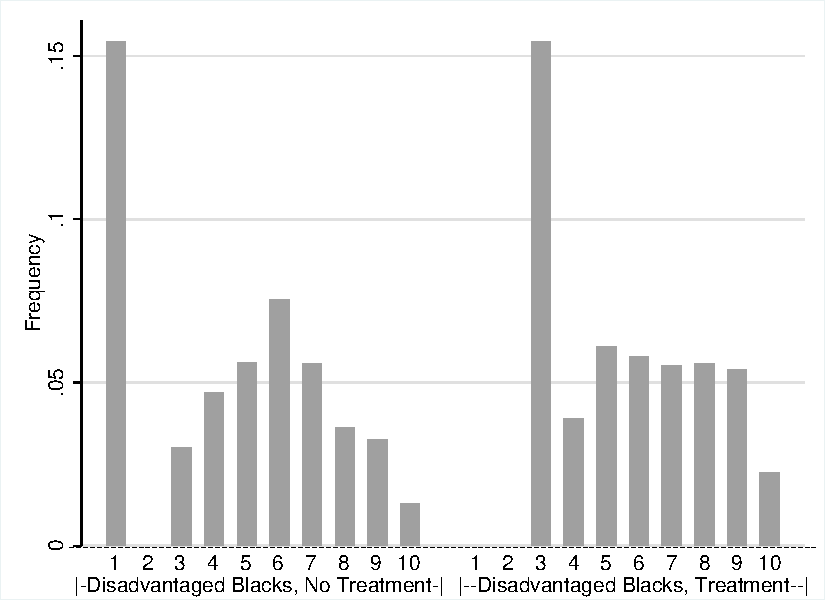
\includegraphics{female1_perry}}} \\
         \subfloat[How the Black Fit into the White Distribution at Age 27, by decile]{
                \scalebox{0.75}{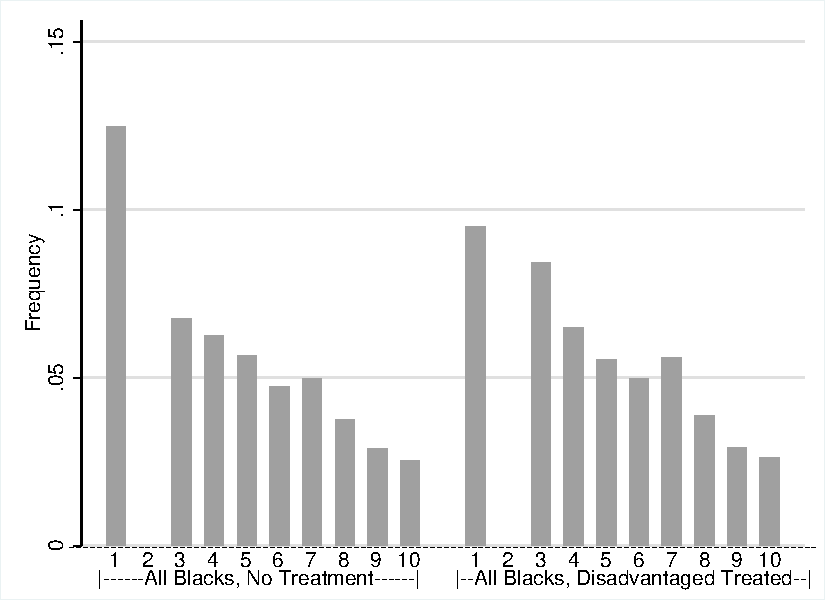
\includegraphics{female2_perry}}} \\
\end{center}
{\scriptsize {\bfseries Notes: } \raggedright The black disadvantaged group is composed of black individuals that satisfy the following criteria: 1) at least one older sibling; 2) IQ score lower than 85; 3) SES index at most 11. All the criteria are measured at age 3. The latter two criteria are approximated as in \citet{heckman2010analyzing}. The black non-disadvantaged are the individuals that violated some of the three criteria above. Black and white are representative of the cohort aged 14-22 in 1979. The left hand side plots consider the cases of the No Action Scenario (Scenario 1): the Perry Program does not influence adult outcomes. The right hand side plots consider cases of the Counter-factual Scenario (Scenario 2): we apply the gender-specific treatment effects of the Perry Program to the disadvantaged black population. We use the treatment effects calculated by \citet{heckman2010analyzing}. 
}
\end{figure}


\begin{figure} \begin{center}\centering
        \caption{Perry Birth Cohort: Total Annual Earnings, Females Age 40}
        \label{female_earn_decile2}\vspace{0.2cm}
         \subfloat[How the Black Disadvantaged Fit into the Black Distribution at Age 40, by decile]{
                \scalebox{0.75}{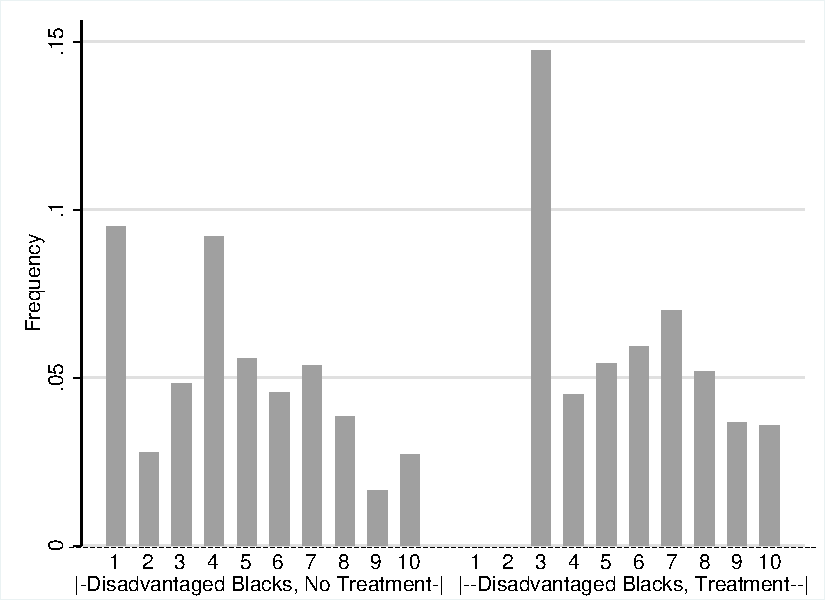
\includegraphics{female3_perry}}} \\
         \subfloat[How the Black Fit into the White Distribution at Age 40, by decile]{
                \scalebox{0.75}{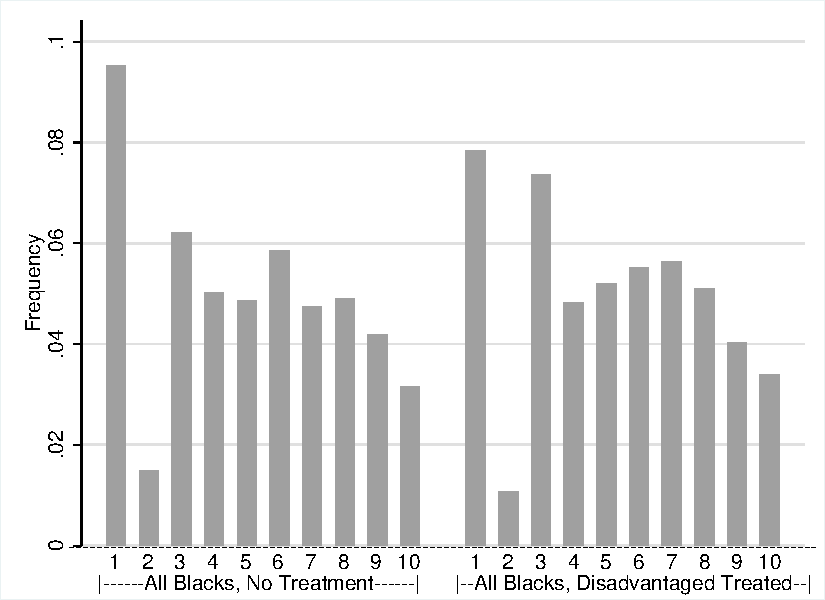
\includegraphics{female4_perry}}} \\     
\end{center}
{\scriptsize {\bfseries Notes: } \raggedright The black disadvantaged group is composed of black individuals that satisfy the following criteria: 1) at least one older sibling; 2) IQ score lower than 85; 3) SES index at most 11. All the criteria are measured at age 3. The latter two criteria are approximated as in \citet{heckman2010analyzing}. The black non-disadvantaged are the individuals that violated some of the three criteria above. Black and white are representative of the cohort aged 14-22 in 1979. The left hand side plots consider the cases of the No Action Scenario (Scenario 1): the Perry Program does not influence adult outcomes. The right hand side plots consider cases of the Counter-factual Scenario (Scenario 2): we apply the gender-specific treatment effects of the Perry Program to the disadvantaged black population. We use the treatment effects calculated by \citet{heckman2010analyzing}. 
}
\end{figure}


\begin{figure} \begin{center}\centering
        \caption{Perry Birth Cohort: Total Annual Earnings, Males Age 27}
        \label{male_earn_decile1}\vspace{0.2cm}
        
         \subfloat[How the Black Disadvantaged Fit into the Black Distribution at Age 27, by decile]{
                \scalebox{0.75}{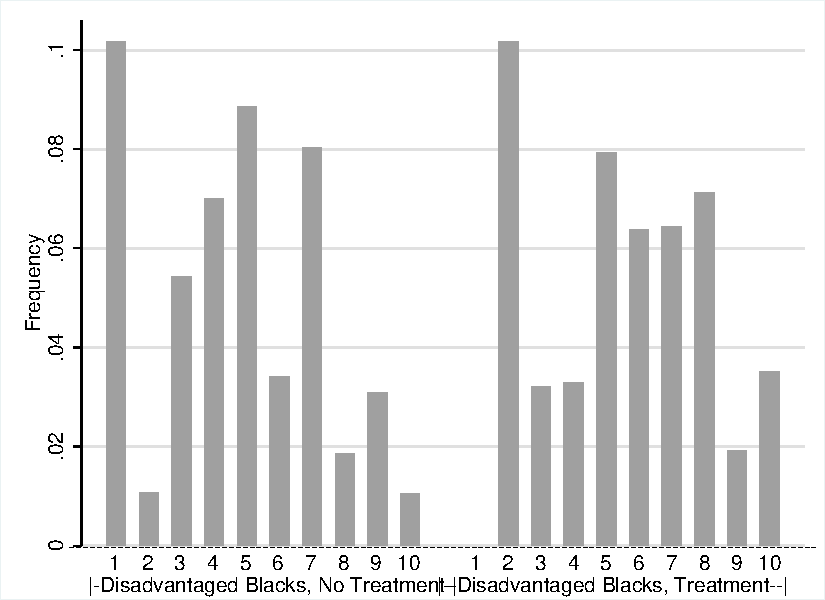
\includegraphics{male1_perry}}} \\
         \subfloat[How the Black Fit into the White Distribution at Age 27, by decile]{
                \scalebox{0.75}{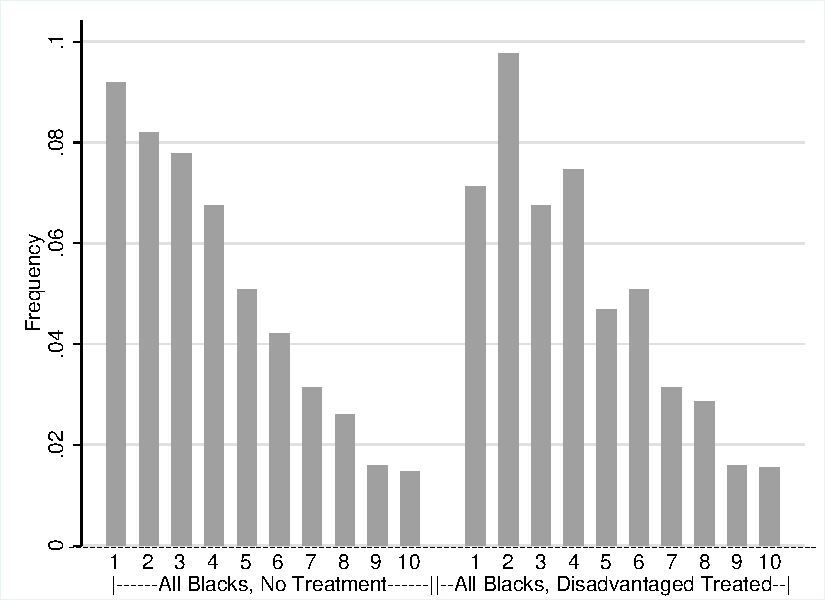
\includegraphics{male2_perry}}} \\
\end{center}
{\scriptsize {\bfseries Notes: } \raggedright The black disadvantaged group is composed of black individuals that satisfy the following criteria: 1) at least one older sibling; 2) IQ score lower than 85; 3) SES index at most 11. All the criteria are measured at age 3. The latter two criteria are approximated as in \citet{heckman2010analyzing}. The black non-disadvantaged are the individuals that violated some of the three criteria above. Black and white are representative of the cohort aged 14-22 in 1979. The left hand side plots consider the cases of the No Action Scenario (Scenario 1): the Perry Program does not influence adult outcomes. The right hand side plots consider cases of the Counter-factual Scenario (Scenario 2): we apply the gender-specific treatment effects of the Perry Program to the disadvantaged black population. We use the treatment effects calculated by \citet{heckman2010analyzing}. 
}
\end{figure}



\begin{figure} \begin{center}\centering
        \caption{Perry Birth Cohort: Total Annual Earnings, Males Age 40}
        \label{male_earn_decile2}\vspace{0.2cm}

         \subfloat[How the Black Disadvantaged Fit into the Black Distribution at Age 40, by decile]{
                \scalebox{0.75}{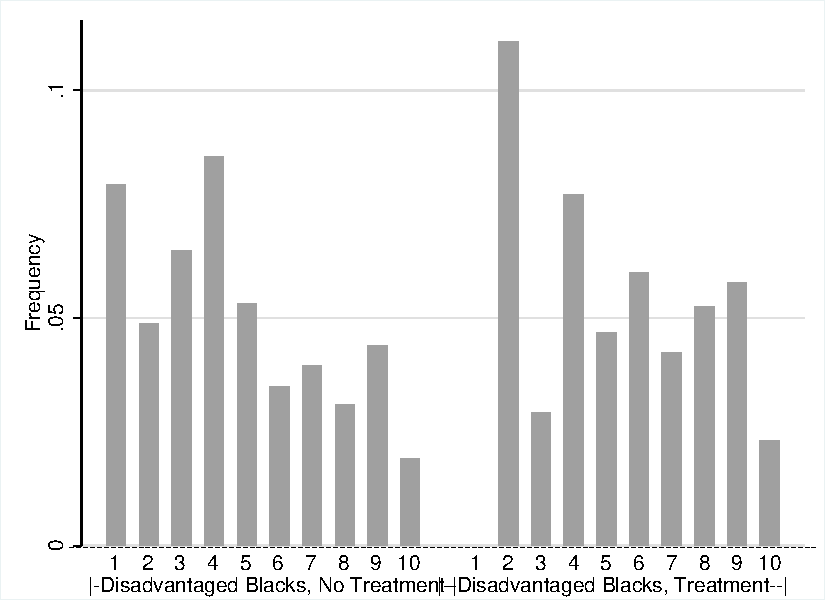
\includegraphics{male3_perry}}} \\
         \subfloat[How the Black Fit into the White Distribution at Age 40, by decile]{
                \scalebox{0.75}{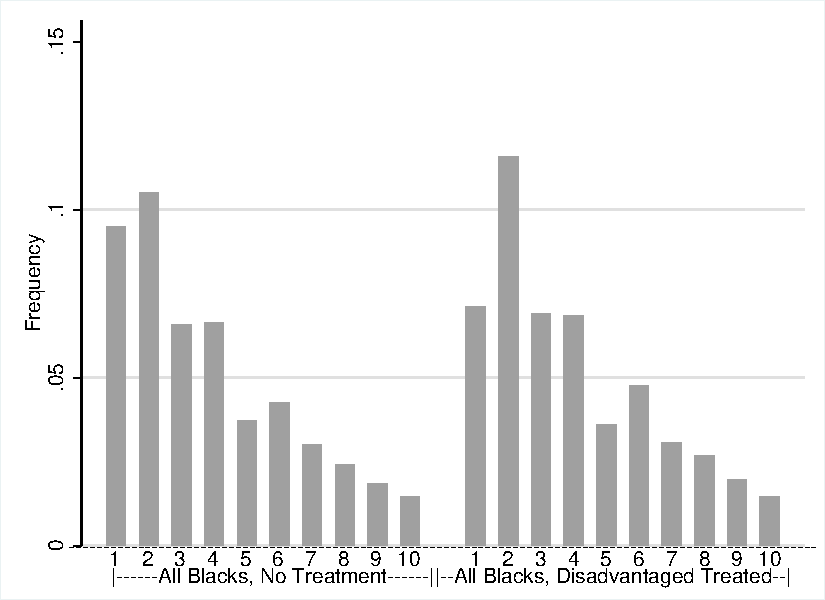
\includegraphics{male4_perry}}} \\ 
\end{center}
{\scriptsize {\bfseries Notes: } \raggedright The black disadvantaged group is composed of black individuals that satisfy the following criteria: 1) at least one older sibling; 2) IQ score lower than 85; 3) SES index at most 11. All the criteria are measured at age 3. The latter two criteria are approximated as in \citet{heckman2010analyzing}. The black non-disadvantaged are the individuals that violated some of the three criteria above. Black and white are representative of the cohort aged 14-22 in 1979. The left hand side plots consider the cases of the No Action Scenario (Scenario 1): the Perry Program does not influence adult outcomes. The right hand side plots consider cases of the Counter-factual Scenario (Scenario 2): we apply the gender-specific treatment effects of the Perry Program to the disadvantaged black population. We use the treatment effects calculated by \citet{heckman2010analyzing}. 
}
\end{figure}


\restoregeometry

\section{The Abecedarian Project} \label{sec:ABC}

The Carolina Abecedarian Project (ABC) ran between 1972 and the early 1980s in Chapel Hill, North Carolina. The intervention randomly assigned children to control and treatment groups in two separate stages: one during preschool years and another during primary school years. We consider the preschool treatment. This provided 117 children with high quality center-based care from birth to age five. Nearly all of the ABC children were black. Actually, we disregard the non-African-American children to keep the sample comparable with Perry. They were followed up until age 34. 

Admission to the program took place over a $5$-year period resulting in four cohorts of approximately $28$ children each. Children were recruited in four separate waves by eliciting referrals from local community organizations such as prenatal clinics, hospitals, and social services \citep{Breitmayer_Ramey_1986_CD}. Families whose children appeared healthy and free from biological conditions that could be associated with mental, sensory, or motor disabilities were contacted (\citet{Ramey_Campbell_1984}). Once a potential candidate was identified, a High-Risk Index (HRI) was accessed to determine preliminary eligibility. This index was computed from $13$ socio-economic factors as described in \citet{Ramey_Smith_1977_AJMD}.
Each family's value was compared to a cutoff value to determine eligibility (the family was included if their index was greater than $11$). Final eligibility was determined after an interview with the mothers of the candidates, where data on demographic characteristics of their families was collected. In addition, maternal intelligence was assessed using the Wechsler Adult Intelligence Scale (WAIS, Wechsler 1955). The selection process took place either before or shortly after the birth of the subject child.

A total of $122$ families eligible families (combining all waves) were invited to enroll the program; however $121$ agreed to participate.
Among those who complied, one mother experience a miscarriage. The final randomized set consists of $120$ families associated with $122$ children. The first randomization, which is the one important for our study, was performed immediately after each cohort was formed; all $122$ children were included. According to \citet{Ramey_Campbell_1984}, the initial $122$ children were matched in pairs by ``identifying most similar pairs in the High-Risk Index''. \citet{Breitmayer_Ramey_1986_CD} have a more detailed description: ``qualifying families were first pair matched on sex of the child, maternal IQ, number of siblings and High-Risk Index score''. The precise matched pairs are unknown. Subsequently, the matched children were randomly assigned to either the educationally treated group or the control group within each pair. The final treatment status in the first randomization is known for $118$ out of $122$ children; $61$ were assigned to the Early Childhood Intervention (also known as day-care treatment group) and $57$ to the control group.

Before treatment began $11$ children were dropped, reducing the number from $122$ to $111$. Out of the $120$ families that initially participated before the randomization, $8$ families declined participation after learning their treatment assignment ($7$ families from the treatment group and $1$ family from control). Two participants previously assigned to the control group were swapped to the treatment group at the request of the local authorities,
as their lives were threatened due to poor health conditions. Finally, one child was excluded after being diagnosed with idiopathic moderate retardation associated with a seizure disorder (\citet{Campbell_Ramey_1995_AERJ}). None of these $11$ children were included in the final sample of Abecedarian project. The final base sample included $109$ families to whom $111$ children were born, $57$ of whom were assigned to treatment group and $54$ were assigned to the control group.

Data on cognitive skills, noncognitive skills, health, achievement, and behavior was collected at multiple stages from birth until the end of the school age. More follow-ups occurred at age 12, age 15, age 21 and age 30. Finally, more data was collected based on governmental records, such as criminal behavior. Attrition at the follow-ups was fairly minimal. In fact most of the attrition occurred before or during the treatment stages. 

\subsection{A Nationally Representative Comparable Sample: the PSID}
Beginning in 1968, the Panel Study of Income Dynamics (PSID) followed 18,000 individuals from 5,000 families living in the United States. The study collected information on these individuals and their descendants every year between 1968 and 1999, after which data collection occured biannually. The data includes measures of: employment, income, wealth, expenditures, health, marriage, childbearing, child development and education. We construct a subsample of the PSID comparable to the cohort to which the ABC sample belonged.

Additionally, we identify a subsample of disadvantaged blacks that satisfy the ABC eligibility criteria. To identify this subsample, we reconstruct the ABC High-Risk Index and flag blacks with an index exceeding 11. A few components to the risk index have no corresponding PSID variable. In the ABC data, we estimate linear models of low sibling IQ, in need of professional help and special circumstances with mother's age at birth, number of siblings, absent father, lack of maternal relatives and an indicator for welfare. We apply this model to the PSID to generate the missing components of the risk index. Additionally, we perform within PSID sample regressions of father has unstable work, father's and mother's education, mother's age at birth and family unit Head IQ on absent father, lack of relatives in the area, an indicator for receiving welfare and income at birth. We use the parameters from this regression to impute the missing data of the regressands. Following these imputation steps, we construct the ABC High-Risk Index. Tables \ref{tab:tabfem_abc} and \ref{tab:tabmal_abc} compares the ABC sample to the PSID subsample of disadvantaged blacks satisfying the Risk-Index criterium for ABC eligibility.  

\subsection{Results}
It is important to note that our construction of the risk index relies on some strong assumptions regarding the implementation of the calculations of the index. Using this construction, roughly half of the black population would have been eligible for the program at the time. We focus on 4 outcomes: (i) 4 year college degree at 40; (ii) employed at 30; (iii) high-school school graduation 30; (iv) earnings at 30 (in year 2010 dollars). Tables \ref{tab:tabfem_abc} and \ref{tab:tabmal_abc} show the results. First, we display the number of individuals in the ABC and corresponding PSID samples. Then we show how many people the PSID samples represent in the population. Second, we display the pretreatment variables to show how well the PSID disadvantaged sample compares to the ABC sample. Third, we show the adult outcomes for both ABC (treatment and control) and the PSID. For the PSID we display the actual outcomes and the outcomes when the treatment effects are applied as described in Section \ref{sec:Meth}. Finally, we show the intra-black and the black-white gaps under Scenarios 1 and 2. The percent change in the gaps between scenarios is also presented. Figures \ref{female_earn_decile_abc} and \ref{male_earn_decile_abc} compare how the treated groups (we consider disadvantaged blacks and all blacks) would  change their position within the earnings distributions of the untreated groups (we consider non-disadvantaged blacks and whites) after being treated.


\clearpage
\newgeometry{left=1.3cm,right=1.3cm,top=1.3cm,bottom=1.5cm}
% matrix: A_0 file: tabfem_abc.tex   3 Jul 2014 11:43:26
\begin{table}[htbp]
\caption{\label{tab:tabfem_abc} Hypothetical Extension of the Carolina Abecedarian Program to the Disadvantaged Black, Female}\medskip
\footnotesize  \begin{center} \begin{tabular}{lcccccccc}  \hline \hline    
&\multicolumn{2}{c}{ABC Individuals} &\multicolumn{6}{c}{PSID Individuals}  \\[0.05cm]  \cline{2-3} \cline{5-9}   
 & \multicolumn{2}{c}{      }  & \multicolumn{2}{c}{Disadvantaged}  & \multicolumn{1}{c}{Non-disadv.}  & \multicolumn{2}{c}{All Blacks}  & \multicolumn{1}{c}{All Whites} \\  & \multicolumn{1}{c}{Treatment}  & \multicolumn{1}{c}{Control}  & \multicolumn{2}{c}{Blacks}  & \multicolumn{1}{c}{Blacks}  & \multicolumn{2}{c}{ } \\   \hline   
\textbf{(a)} Sample Size &31&           32& \multicolumn{2}{c}{          105} & \multicolumn{1}{c}{           97} &
\multicolumn{2}{c}{          202} &
\multicolumn{1}{c}{          349} 
 \\[0.05cm] 
\ \ \ \ \ Population Represented &.&            .& \multicolumn{2}{c}{      479,348} & \multicolumn{1}{c}{      432,945} &
\multicolumn{2}{c}{      912,293} &
\multicolumn{1}{c}{    5,165,944} 
 \\[0.2cm] \hline
\textbf{(b) Pre-Treatment Variables}  \\[0.2cm] 
Mother's years of schooling &        10.58 &         9.84 & \multicolumn{2}{c}{        11.54} &
\multicolumn{1}{c}{        12.21} &
\multicolumn{2}{c}{        11.86} &
\multicolumn{1}{c}{        12.99} 
 \\[0.05cm]  
 & (        1.69) & (        2.08) & \multicolumn{2}{c}{(        2.00)} &
\multicolumn{1}{c}{(        1.92)} &
\multicolumn{2}{c}{(        1.99)} &
\multicolumn{1}{c}{(        2.07)} 
 \\[0.2cm]  
Number of Siblings at Birth &         0.45 &         0.66 & \multicolumn{2}{c}{         2.01} &
\multicolumn{1}{c}{         2.21} &
\multicolumn{2}{c}{         2.10} &
\multicolumn{1}{c}{         1.01} 
 \\[0.05cm]  
 & (        0.72) & (        1.10) & \multicolumn{2}{c}{(        2.26)} &
\multicolumn{1}{c}{(        3.32)} &
\multicolumn{2}{c}{(        2.82)} &
\multicolumn{1}{c}{(        1.12)} 
 \\[0.2cm]  
Father Absent at Birth &         0.77 &         0.69 & \multicolumn{2}{c}{         0.89} &
\multicolumn{1}{c}{         0.24} &
\multicolumn{2}{c}{         0.58} &
\multicolumn{1}{c}{         0.16} 
 \\[0.05cm]  
 & (        0.43) & (        0.47) & \multicolumn{2}{c}{(        0.32)} &
\multicolumn{1}{c}{(        0.43)} &
\multicolumn{2}{c}{(        0.49)} &
\multicolumn{1}{c}{(        0.37)} 
 \\[0.2cm]  
\hline
\textbf{(c) Adult Outcomes} &Treated &Control  &Actual &If Treated &Actual &Actual &Disadv. &Actual \\[0.02cm] 
 & &  && & & & Treated & \\[0.2cm] 
4 Year College Degree at 30 &         0.20 &         0.00 &         0.10 &         0.26 &         0.23 &         0.16 &         0.25 &         0.35 \\[0.05cm]  
 & (        0.41) & (        0.00) & (        0.31) & (        0.31) & (        0.42) & (        0.37) & (        0.37) & (        0.48)   \\[0.2cm]  
Employed at 30 &         0.88 &         0.71 &         0.58 &         0.65 &         0.84 &         0.71 &         0.74 &         0.76 \\[0.05cm]  
 & (        0.33) & (        0.46) & (        0.49) & (        0.49) & (        0.36) & (        0.46) & (        0.45) & (        0.43)   \\[0.2cm]  
High School Grad at 30 &         0.76 &         0.54 &         0.70 &         0.86 &         0.89 &         0.79 &         0.87 &         0.93 \\[0.05cm]  
 & (        0.44) & (        0.51) & (        0.46) & (        0.46) & (        0.32) & (        0.41) & (        0.40) & (        0.26)   \\[0.2cm]  
Earnings at 30 (in 2010 dollars) &       29,040 &       24,879 &       18,697 &       19,629 &       27,844 &       22,918 &       23,420 &       28,913 \\[0.05cm]  
 & (      27,679) & (      22,152) & (      16,221) & (      16,221) & (      18,195) & (      17,756) & (      17,642) & (      24,938)   \\[0.2cm]  
\hline \hline
\textbf{(d) Gaps Applying ABC} & \multicolumn{2}{c}{\textbf{Scenario 1:}} &  &\multicolumn{4}{c}{\textbf{Scenario 2:}}   \\[0.2cm]  
 Pop. getting the program: & \multicolumn{2}{c}{No Action}   &  &\multicolumn{4}{c}{Disadvantaged Blacks are Treated}   \\[0.02cm]  
Cost of Intervention (2010 Mill.) &\multicolumn{2}{c}{ 0 } &
 &\multicolumn{4}{c}{      36,881} &
 \\[0.2cm]  
\hline
&Intra-Black &Black-White & &Intra-Black &Change &Black-White &Change  \\[0.02cm] 
&Gap &Gap & &Gap &in Gap &Gap &in Gap  \\[0.01cm] 
\hline
4 Year College Degree at 30 &        0.13&        0.18&&       -0.03&        -123\% &        0.10&         -46\% &
 \\[0.2cm]  
Employed at 30 &        0.26&        0.05&&        0.20&         -24\% &        0.02&         -64\% &
 \\[0.2cm]  
High School Grad at 30 &        0.19&        0.14&&        0.02&         -88\% &        0.05&         -62\% &
 \\[0.2cm]  
Earnings at 30 (in 2010 dollars) &       9,148&       5,996&&       8,215&         -10\% &       5,494&          -8\% &
 \\[0.2cm]  
  \hline \hline    \end{tabular}
 \end{center} 
       {\scriptsize  
       {\raggedright 
 {\bfseries Notes:} The data on the ABC  subjects come from the Carolina Abecedarian Program dataset. For all other  groups we rely on data in the PSID for individuals born between 1972 and 1977.   The PSID weights are used to make each sample representative  of its correlative in the population. Disadvantaged blacks meet the  ABC eligibility criteria. Non-disadvantaged blacks are those that do  not meet ABC eligibility. All blacks include disadvantaged and non- disadvantaged blacks and represent the U.S. population of blacks. All  whites represents the entire U.S. population of whites. The first row in  Panel (a) shows the sample sizes. The first two columns for the treatment  and control individuals and the last four columns for the different categories  of the PSID. The second row of Panel (a) shows how many individuals are  represented by the sample that we consider. Panel (b) describes the pre-  treatment variables for ABC and the PSID. The pretreatment characteristics  of the control and treatment groups in ABC are similar because of the  randomized nature of the experiment; our exercise gains validity if these  are similar to the characteristics of the disadvantaged group in the PSID  which are shown in the third column. The rest of the columns in Panel (b)  describe the pretreatment variables for the rest of the groups. Panel (c)  describes adult outcomes. The first two columns do so for ABC. The third column  describes the actual adult outcomes for the disadvantaged black in the PSID,  while column four displays analogous information for the outcomes when the  treatment effects of ABC are applied. The fifth column presents adult outcomes  for the non-disadvantaged blacks. The sixth and seventh columns present adult outcomes before  and after the treatment effects of ABC are applied. The  eighth shows adult outcomes for whites. Panel (d) describes the outcome gaps.  Scenario 1 is the baseline scenario, where ABC is not available. In Scenario 2  the ABC Program is available to all disadvantaged blacks. The intra- black gap measures the difference in adult outcomes between the non- disadvantaged black population and the disadvantaged black population.  The black-white gap compares the difference in adult outcomes between the  whole black population and the whole white population. The first two columns  show the gaps under Scenario 1. The last four columns present the gaps under  Scenario 2 and the percent changes from the gaps under Scenario 1. } } 
 \end{table}

% matrix: A_1 file: tabmal_abc.tex   3 Jul 2014 11:43:26
\begin{table}[htbp]
\caption{\label{tab:tabmal_abc} Hypothetical Extension of the Carolina Abecedarian Program to the Disadvantaged Black, Male}\medskip
\footnotesize  \begin{center} \begin{tabular}{lcccccccc}  \hline \hline    
&\multicolumn{2}{c}{ABC Individuals} &\multicolumn{6}{c}{PSID Individuals}  \\[0.05cm]  \cline{2-3} \cline{5-9}   
 & \multicolumn{2}{c}{    }  & \multicolumn{2}{c}{Disadvantaged}  & \multicolumn{1}{c}{Non-disadv.}  & \multicolumn{2}{c}{All Blacks}  & \multicolumn{1}{c}{All Whites} \\  & \multicolumn{1}{c}{Treatment}  & \multicolumn{1}{c}{Control}  & \multicolumn{2}{c}{Blacks}  & \multicolumn{1}{c}{Blacks}  & \multicolumn{2}{c}{ } \\   \hline   
\textbf{(a)} Sample Size &30&           25& \multicolumn{2}{c}{           50} & \multicolumn{1}{c}{           93} &
\multicolumn{2}{c}{          143} &
\multicolumn{1}{c}{          336} 
 \\[0.05cm] 
\ \ \ \ \ Population Represented &.&            .& \multicolumn{2}{c}{      242,574} & \multicolumn{1}{c}{      457,383} &
\multicolumn{2}{c}{      699,957} &
\multicolumn{1}{c}{    4,952,654} 
 \\[0.2cm] \hline
\textbf{(b) Pre-Treatment Variables}  \\[0.2cm] 
Mother's years of schooling &        10.30 &         9.92 & \multicolumn{2}{c}{        11.47} &
\multicolumn{1}{c}{        12.43} &
\multicolumn{2}{c}{        12.10} &
\multicolumn{1}{c}{        12.95} 
 \\[0.05cm]  
 & (        1.78) & (        1.75) & \multicolumn{2}{c}{(        1.08)} &
\multicolumn{1}{c}{(        1.74)} &
\multicolumn{2}{c}{(        1.61)} &
\multicolumn{1}{c}{(        2.01)} 
 \\[0.2cm]  
Number of Siblings at Birth &         0.60 &         0.88 & \multicolumn{2}{c}{         1.61} &
\multicolumn{1}{c}{         1.00} &
\multicolumn{2}{c}{         1.21} &
\multicolumn{1}{c}{         0.94} 
 \\[0.05cm]  
 & (        1.10) & (        1.42) & \multicolumn{2}{c}{(        1.68)} &
\multicolumn{1}{c}{(        1.11)} &
\multicolumn{2}{c}{(        1.37)} &
\multicolumn{1}{c}{(        1.17)} 
 \\[0.2cm]  
Father Absent at Birth &         0.77 &         0.60 & \multicolumn{2}{c}{         0.94} &
\multicolumn{1}{c}{         0.20} &
\multicolumn{2}{c}{         0.45} &
\multicolumn{1}{c}{         0.08} 
 \\[0.05cm]  
 & (        0.43) & (        0.50) & \multicolumn{2}{c}{(        0.24)} &
\multicolumn{1}{c}{(        0.40)} &
\multicolumn{2}{c}{(        0.50)} &
\multicolumn{1}{c}{(        0.28)} 
 \\[0.2cm]  
\hline
\textbf{(c) Adult Outcomes} &Treated &Control  &Actual &If Treated &Actual &Actual &Disadv. &Actual \\[0.02cm] 
 & &  && & & & Treated & \\[0.2cm] 
4 Year College Degree at 30 &         0.26 &         0.05 &         0.06 &         0.30 &         0.21 &         0.16 &         0.25 &         0.30 \\[0.05cm]  
 & (        0.45) & (        0.22) & (        0.23) & (        0.23) & (        0.41) & (        0.36) & (        0.36) & (        0.46)   \\[0.2cm]  
Employed at 30 &         0.89 &         0.62 &         0.80 &         1.05 &         0.89 &         0.86 &         0.95 &         0.91 \\[0.05cm]  
 & (        0.32) & (        0.50) & (        0.40) & (        0.40) & (        0.31) & (        0.34) & (        0.35) & (        0.28)   \\[0.2cm]  
High School Grad at 30 &         0.70 &         0.52 &         0.83 &         1.00 &         0.93 &         0.89 &         0.96 &         0.90 \\[0.05cm]  
 & (        0.47) & (        0.51) & (        0.37) & (        0.37) & (        0.26) & (        0.31) & (        0.31) & (        0.30)   \\[0.2cm]  
Earnings at 30 (in 2010 dollars) &       40,784 &       25,438 &       21,019 &       44,380 &       36,842 &       31,280 &       39,491 &       52,262 \\[0.05cm]  
 & (      41,924) & (      32,369) & (      14,061) & (      14,061) & (      19,486) & (      19,308) & (      18,130) & (      37,151)   \\[0.2cm]  
\hline \hline
\textbf{(d) Gaps Applying ABC} & \multicolumn{2}{c}{\textbf{Scenario 1:}} &  &\multicolumn{4}{c}{\textbf{Scenario 2:}}   \\[0.2cm]  
 Pop. getting the program: & \multicolumn{2}{c}{No Action}   &  &\multicolumn{4}{c}{Disadvantaged Blacks are Treated}   \\[0.02cm]  
Cost of Intervention (2010 Mill.) &\multicolumn{2}{c}{ 0 } &
 &\multicolumn{4}{c}{      18,663} &
 \\[0.2cm]  
\hline
&Intra-Black &Black-White & &Intra-Black &Change &Black-White &Change  \\[0.02cm] 
&Gap &Gap & &Gap &in Gap &Gap &in Gap  \\[0.01cm] 
\hline
4 Year College Degree at 30 &        0.16&        0.14&&       -0.09&        -155\% &        0.05&         -63\% &
 \\[0.2cm]  
Employed at 30 &        0.09&        0.05&&       -0.15&        -268\% &       -0.03&        -165\% &
 \\[0.2cm]  
High School Grad at 30 &        0.10&        0.01&&       -0.07&        -174\% &       -0.05&        -734\% &
 \\[0.2cm]  
Earnings at 30 (in 2010 dollars) &      15,823&      20,982&&      -7,539&        -148\% &      12,771&         -39\% &
 \\[0.2cm]  
  \hline \hline    \end{tabular}
 \end{center} 
       {\scriptsize  
       {\raggedright 
 {\bfseries Notes:} The data on the ABC  subjects come from the Carolina Abecedarian Program dataset. For all other  groups we rely on data in the PSID for individuals born between 1972 and 1977.   The PSID weights are used to make each sample representative  of its correlative in the population. Disadvantaged blacks meet the  ABC eligibility criteria. Non-disadvantaged blacks are those that do  not meet ABC eligibility. All blacks include disadvantaged and non- disadvantaged blacks and represent the U.S. population of blacks. All  whites represents the entire U.S. population of whites. The first row in  Panel (a) shows the sample sizes. The first two columns for the treatment  and control individuals and the last four columns for the different categories  of the PSID. The second row of Panel (a) shows how many individuals are  represented by the sample that we consider. Panel (b) describes the pre-  treatment variables for ABC and the PSID. The pretreatment characteristics  of the control and treatment groups in ABC are similar because of the  randomized nature of the experiment; our exercise gains validity if these  are similar to the characteristics of the disadvantaged group in the PSID  which are shown in the third column. The rest of the columns in Panel (b)  describe the pretreatment variables for the rest of the groups. Panel (c)  describes adult outcomes. The first two columns do so for ABC. The third column  describes the actual adult outcomes for the disadvantaged black in the PSID,  while column four displays analogous information for the outcomes when the  treatment effects of ABC are applied. The fifth column presents adult outcomes  for the non-disadvantaged blacks. The sixth and seventh columns present adult outcomes before  and after the treatment effects of ABC are applied. The  eighth shows adult outcomes for whites. Panel (d) describes the outcome gaps.  Scenario 1 is the baseline scenario, where ABC is not available. In Scenario 2  the ABC Program is available to all disadvantaged blacks. The intra- black gap measures the difference in adult outcomes between the non- disadvantaged black population and the disadvantaged black population.  The black-white gap compares the difference in adult outcomes between the  whole black population and the whole white population. The first two columns  show the gaps under Scenario 1. The last four columns present the gaps under  Scenario 2 and the percent changes from the gaps under Scenario 1. } } 
 \end{table}

\restoregeometry

\newgeometry{bottom=2.5cm}
\begin{figure} \begin{center}\centering
        \caption{ABC Birth Cohort: Total Annual Earnings, Females Age 30}
        \label{female_earn_decile_abc}\vspace{0.2cm}
         \subfloat[How the Black Disadvantaged Fit into the Black Distribution at Age 30, by decile]{
                \scalebox{0.75}{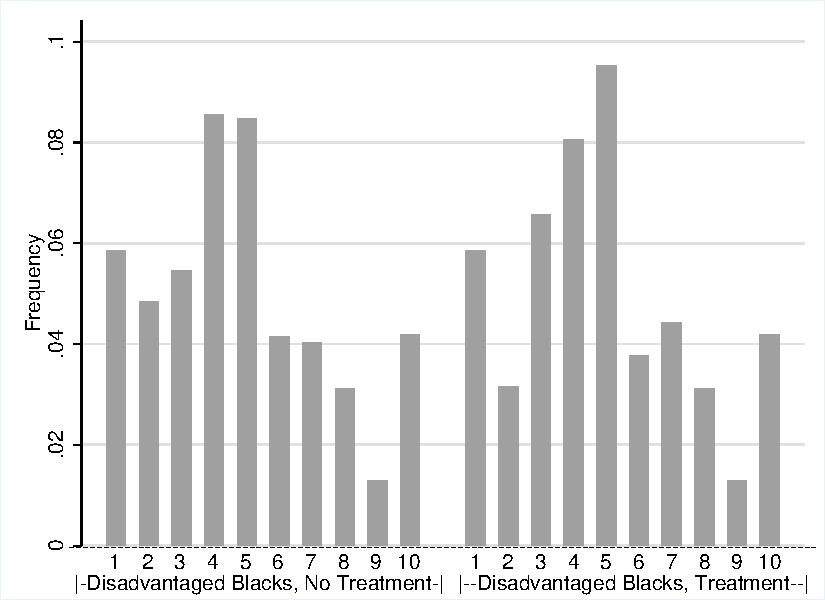
\includegraphics{female3_abc}}} \\
         \subfloat[How the Black Fit into the White Distribution at Age 30, by decile]{
                \scalebox{0.75}{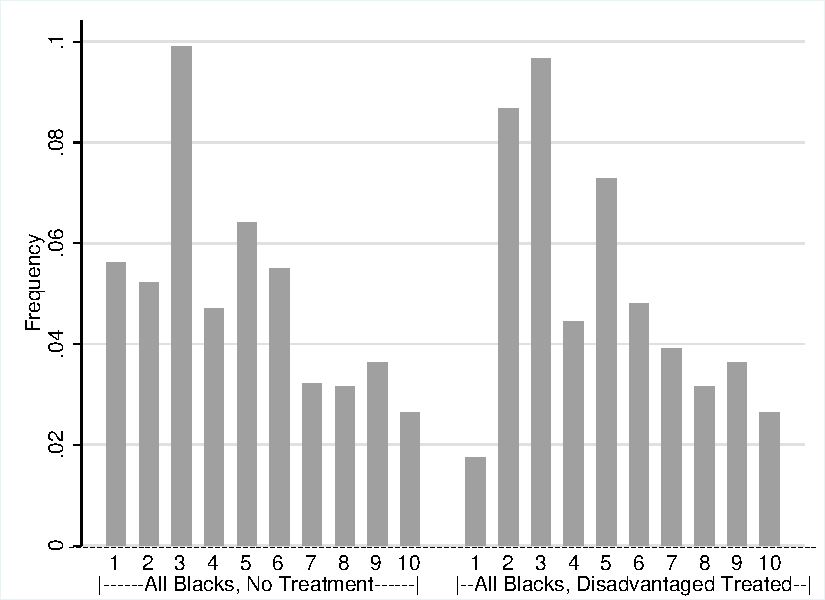
\includegraphics{female4_abc}}} \\     
\end{center}
{\scriptsize {\bfseries Notes: } \raggedright Earnings are three year averages centered at age 30. The black disadvantaged group satisfies the ABC eligibility criteria. The black non-disadvantaged do not satisfy this criteria. Black and white are representative of the cohort born between 1972 and 1977. The left hand side plots consider the cases of the No Action Scenario (Scenario 1): the ABC Program does not influence adult outcomes. The right hand side plots consider cases of the Counter-factual Scenario (Scenario 2): we apply the gender-specific treatment effects of the ABC Program to the disadvantaged black population. We use the treatment effects calculated by \citet{Frances_2013_EJ}.
}
\end{figure}

\begin{figure} \begin{center}\centering
        \caption{ABC Birth Cohort: Total Annual Earnings, Males Age 30}
        \label{male_earn_decile_abc}\vspace{0.2cm}        
         \subfloat[How the Black Disadvantaged Fit into the Black Distribution at Age 30, by decile]{
                \scalebox{0.75}{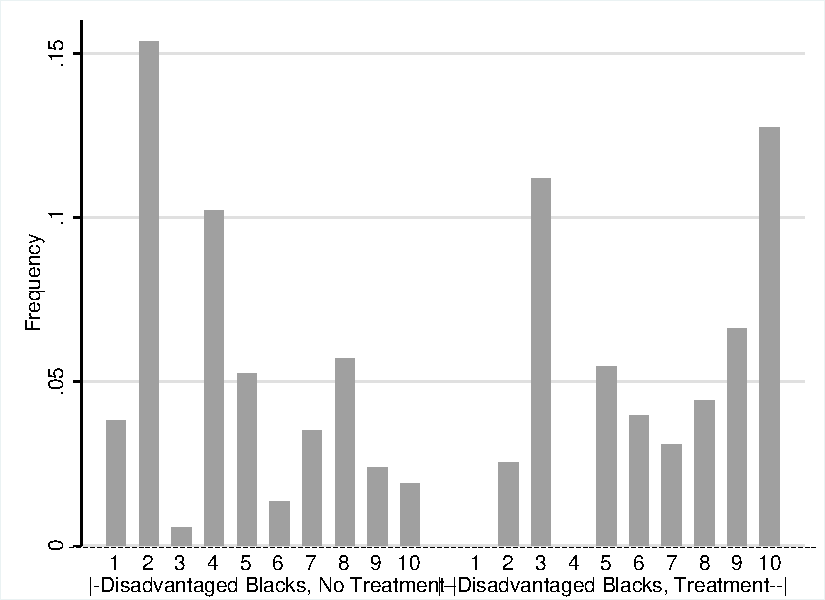
\includegraphics{male3_abc}}} \\
         \subfloat[How the Black Fit into the White Distribution at Age 30, by decile]{
                \scalebox{0.75}{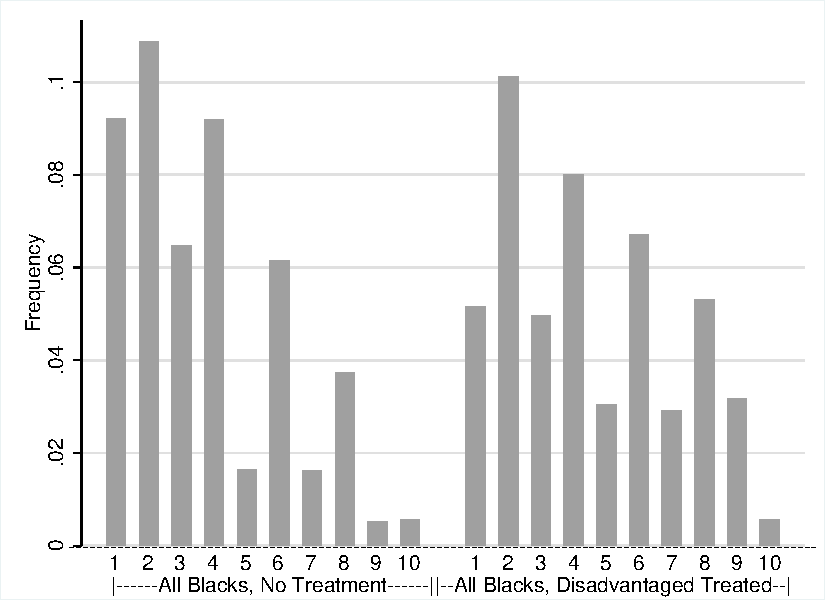
\includegraphics{male4_abc}}} \\
\end{center}
{\scriptsize {\bfseries Notes: } \raggedright Earnings are three year averages centered at age 30. The black disadvantaged group satisfies the ABC eligibility criteria. The black non-disadvantaged do not satisfy this criteria. Black and white are representative of the cohort born between 1972 and 1977. The left hand side plots consider the cases of the No Action Scenario (Scenario 1): the ABC Program does not influence adult outcomes. The right hand side plots consider cases of the Counter-factual Scenario (Scenario 2): we apply the gender-specific treatment effects of the ABC Program to the disadvantaged black population. We use the treatment effects calculated by \citet{Frances_2013_EJ}. 
}
\end{figure}



\restoregeometry

\medskip{}

\newpage
\section{Appendix: The Relative Disadvantage of Perry and ABC Eligible Children} \label{sec:comp}
%We performed a hypothetical exercise where we projected Perry and ABC treatment effects onto eligible children in the population. We then explored the impact of this exercise on outcome gaps between various populations of the same cohort. The Perry cohort was born between 1957 and 1964. The ABC cohort was born between 1972 and 1977. We use nationally representative samples of these cohorts available in the NLSY79 (Perry) and the PSID (ABC) to evaluate outcome gaps in the population. After reconstructing the Perry and ABC risk indices, we mimic their respective eligibility criteria to obtain our disadvantaged samples. It is on these samples that we apply the treatment effects.  

In this section we show how the disadvantaged populations, identified by the Perry or ABC eligibility criteria, compare to the non-disadvantaged populations on a variety of family characteristics. We hope to characterize how disadvantaged are our ``disadvantaged'' populations in terms of maternal education, family income, and number of siblings. In the NLSY79 sample, family income, maternal education, and number of siblings are measured when the child is between 14 and 22 years old. In the PSID, they are measured at birth. The PSID measure of family income is a three year average up until the birth of the child. The NLSY measure of family income covers only one year. 

Table \ref{tab:pretreat}  presents means of these variables across populations in the ABC and Perry cohorts. The Perry eligible, disadvantaged population have mothers with significantly less education than the non-disadvantaged populations. This disadvantage is less pronounced for the ABC eligible, disadvantaged group, whose mothers attend an average of $11.52$ years of school, compared to about $12.3$ and $12.9$ for the remaining black and non-disadvantaged populations. Disadvantaged children, regardless of the corresponding program, tend to have more siblings. Family income largely differentiates ABC eligible, disadvantaged families (\$24,541) from their non-disadvantaged counterparts (\$49,571 for remaining blacks and \$64,434 for all non-disadvantaged). The family income of Perry eligible, disadvantaged families (\$28,010) is similar to their black non-disadvantaged counterparts (\$29,433), but still significantly different from the rest of the population (\$50,467). 

Figures \ref{graph:abc_moedu_b} through \ref{graph:abc_moink_all} show frequencies of family income and mother's education, by block. The ABC eligible, disadvantaged population is rather comparable in mother's years of schooling to the non-disadvantaged populations. The Perry eligible, disadvantaged population is not. The opposite pattern is exhibited for family income, where the ABC eligible, disadvantaged population is strikingly poorer than the non-disadvantaged populations. The Perry eligible, disadvantaged population seems fairly comparable in family income to other blacks and slightly poorer than the rest of the population. 

We attribute the variation in disadvantage across groups in the ABC and Perry cohorts to: (i) the differences in the eligibility criteria and (ii) the differences in the child's age when family characteristics were measured in our PSID and NLSY79 samples. Family income was not included in the Perry socio-economic index. It included maternal education, household density, and father employment status. Thus, the Perry eligibility criteria might select individuals with higher incomes. Relative to the Perry index, the ABC risk index weights mother's education less and includes family income. Thus, the ABC eligibility criteria selects children from less affluent families, but is relatively less restrictive on maternal education. We might also expect the differences in the ages at which we measure mother's education, family income, and number of siblings to explain these patterns. We can most easily predict the impact of measurement age on the number of siblings. We expect this number to be higher for the NLSY79 sample because, the children being 14 to 22, the measure likely captures the maximum number of siblings in their lifetime. 

% matrix: PRE file: pretreat.tex   3 Jul 2014 11:43:29
\begin{table}[htbp]
\caption{\label{tab:pretreat} Comparison of the Pretreatment Variables Across Groups}\medskip
\footnotesize  \begin{center} \begin{tabular}{lcccccc}  \hline \hline    
 \multicolumn{1}{c}{      }  & \multicolumn{3}{c}{Perry Birth Cohort}  & \multicolumn{3}{c}{Abecedarian Birth Cohort} \\  \multicolumn{1}{c}{      }  & \multicolumn{1}{c}{Disadvantaged}  & \multicolumn{1}{c}{Non-Disad.}  & \multicolumn{1}{c}{Non-Disad.}  & \multicolumn{1}{c}{Disadvantaged}  & \multicolumn{1}{c}{Non-Disadv.}  & \multicolumn{1}{c}{Non-Disadv.} \\  \multicolumn{1}{c}{      }  & \multicolumn{1}{c}{Blacks}  & \multicolumn{1}{c}{Blacks}  & \multicolumn{1}{c}{Population}  & \multicolumn{1}{c}{Blacks}  & \multicolumn{1}{c}{Blacks}  & \multicolumn{1}{c}{Population} \\   \hline   
Population  &      751,092 &    3,777,065 &   28,684,543 &      721,922 &      890,328 &   11,484,609 \\[0.1cm]  
Proportion of Total Population &         0.03 &         0.13 &         0.97 &         0.06 &         0.07 &         0.94 \\[0.1cm]  
Mother's years of schooling  &         9.64 &        11.13 &        11.92 &        11.52 &        12.33 &        12.87 \\[0.05cm]  
& (        2.55)& (        2.57)& (        2.44)& (        1.76)& (        1.84)& (        2.07) \\[0.05cm]  
Number of Siblings at Birth  &         5.90 &         4.36 &         3.22 &         1.87 &         1.59 &         1.01 \\[0.05cm]  
& (        3.01)& (        2.87)& (        2.14)& (        2.10)& (        2.53)& (        1.31) \\[0.05cm]  
Family income  &       28,010 &       29,433 &       50,467 &       24,541 &       49,571 &       64,434 \\[0.05cm]  
& (      26,217)& (      30,965)& (      45,671)& (      13,001)& (      20,219)& (      39,442) \\[0.05cm]  
  \hline \hline    \end{tabular}
 \end{center} 
       {\scriptsize  
       {\raggedright 
{\bfseries Notes:} The table shows the means of the variables indicated in the rows for the different groups  indicated in the columns. Standard Deviations are in parenthesis. The NLSY79/PSID weights are used to make each sample representative of its corresponding in the population. Disadvantaged blacks meet the  respective eligibility criteria. (see \citet{Ramey_Smith_1977_AJMD} and \citet{heckman2010analyzing} ). Non-disadvantaged blacks do  not. Non Disadv. Population includes non-disadvantaged blacks and all non-black people.  Family Income is in 2010 dollars. It is measured as a 3-years average around the age of birth on the PSID,   and around age 14-20 in the NLSY. } } 
 \end{table}


%education
\newgeometry{left=1.3cm,right=1.3cm,top=1.3cm,bottom=1.5cm}
\begin{figure} \begin{center}\centering
        \caption{Comparison of Disadvantaged and Non-Disadvantaged Blacks: Years of Mother's Education}
        \label{graph:abc_moedu_b}\vspace{0.2cm}
         \subfloat[ABC Birth Cohort]{
                \scalebox{0.7}{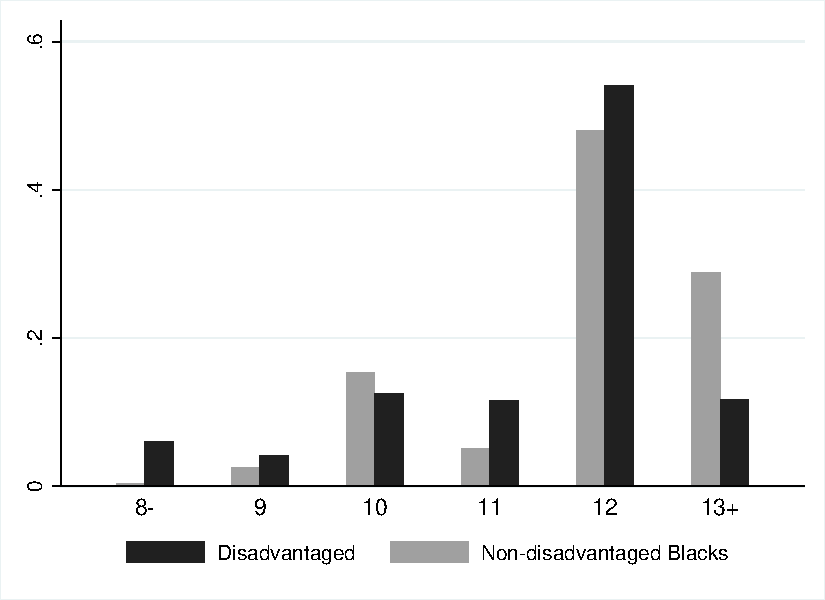
\includegraphics{abc_moedu_b}}}
         \subfloat[Perry Birth Cohort]{
                \scalebox{0.7}{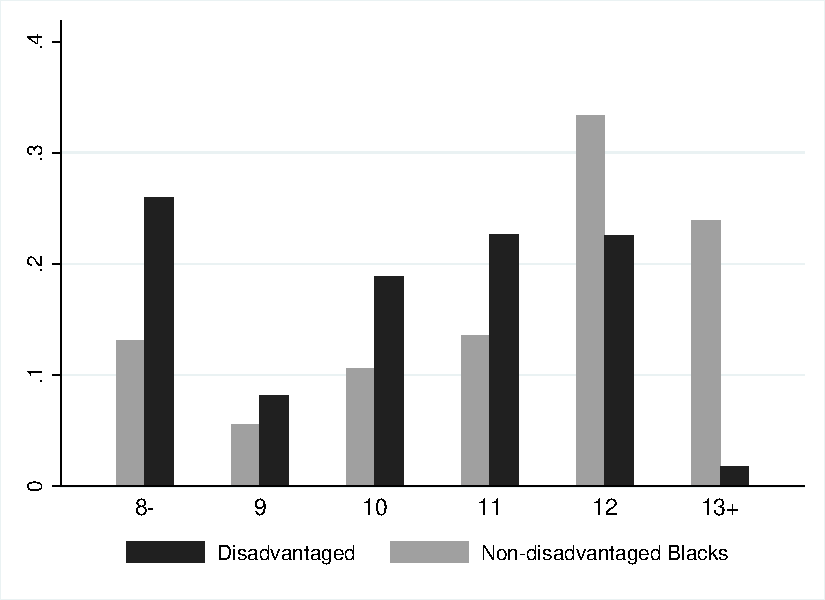
\includegraphics{perry_moedu_b}}} \\
\end{center}
{\scriptsize {\bfseries Notes: } \raggedright 
The figures plot the frequency of mother's years of schooling, by disadvantage status, for the ABC (1972 to 1977) and Perry (1957 to 1964) birth cohorts. For the left plot we use PSID data. 10\% of the cases had the years of education of the mother imputed in that survey. The PSID weights are used to make each sample representative  of its correlative in the population. Disadvantaged blacks meet the  ABC eligibility criteria as described in \citet{Ramey_Smith_1977_AJMD}. For the right plot, we use NLSY79 data. The NLSY weights are used to make each sample representative  of its correlative in the 1979 population. Disadvantaged blacks meet the Perry eligibility criteria as described in \citet{heckman2010analyzing}.
}
\end{figure}

\begin{figure} \begin{center}\centering
        \caption{Comparison of Disadvantaged Blacks and the Rest of the Population: Years of Mother's Education}
        \label{graph:abc_moedu_all}\vspace{0.2cm}
         \subfloat[ABC Birth Cohort]{
                \scalebox{0.7}{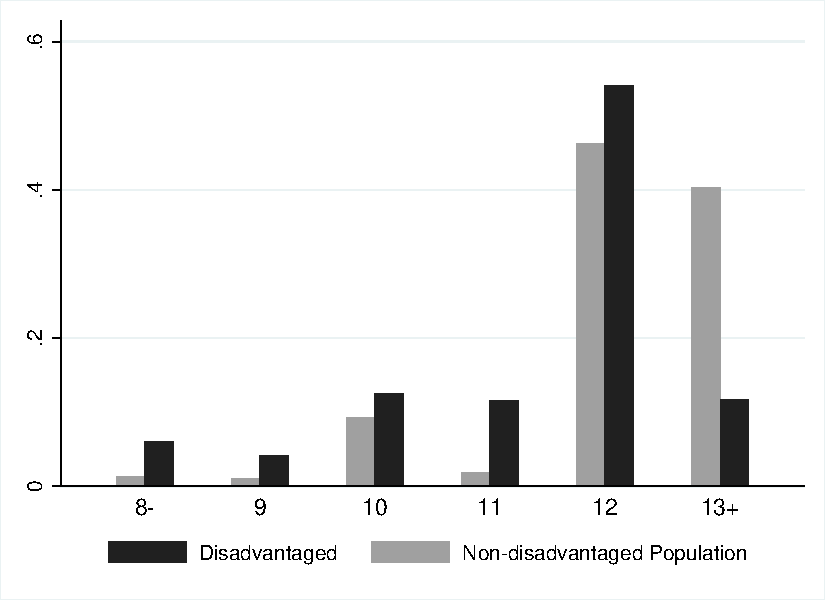
\includegraphics{abc_moedu_all}}}
         \subfloat[Perry Birth Cohort]{
                \scalebox{0.7}{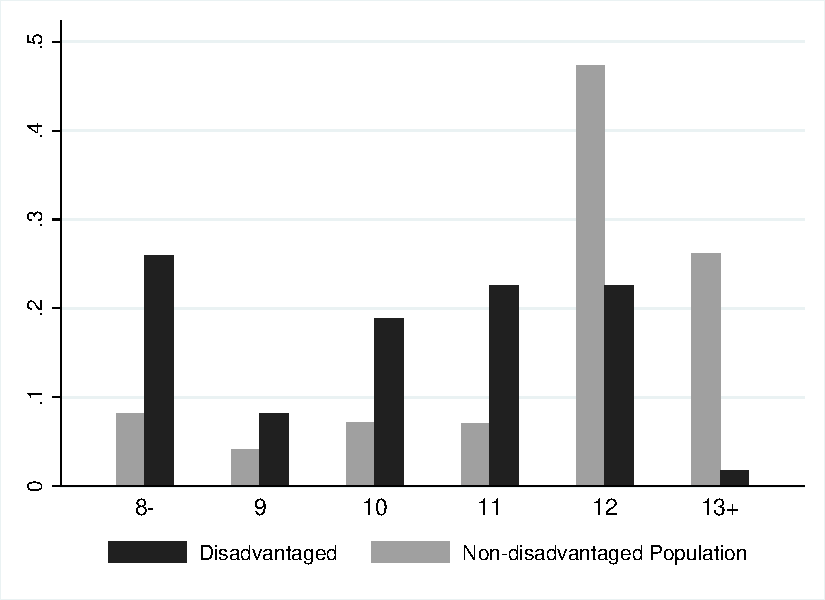
\includegraphics{perry_moedu_all}}} \\
\end{center}
{\scriptsize {\bfseries Notes: } \raggedright 
The figures plot the frequency of mother's years of schooling, by disadvantage status, for the ABC (1972 to 1977) and Perry (1957 to 1964) birth cohorts. For the left plot we use PSID data. 10\% of the cases had the years of education of the mother imputed in that survey. The PSID weights are used to make each sample representative  of its correlative in the population. Disadvantaged blacks meet the  ABC eligibility criteria as described in \citet{Ramey_Smith_1977_AJMD}. For the right plot, we use NLSY79 data. The NLSY weights are used to make each sample representative  of its correlative in the 1979 population. Disadvantaged blacks meet the Perry eligibility criteria as described in \citet{heckman2010analyzing}, and we use the same construction of the eligibility criteria as they do.
}
\end{figure}
\restoregeometry

%income
\newgeometry{left=1.3cm,right=1.3cm,top=1.3cm,bottom=1.3cm}
\begin{figure} \begin{center}\centering
        \caption{Comparison of Disadvantaged and Non-Disadvantaged Blacks: Family Income}
        \label{graph:abc_moink_b}\vspace{0.2cm}
         \subfloat[ABC Birth Cohort]{
                \scalebox{0.7}{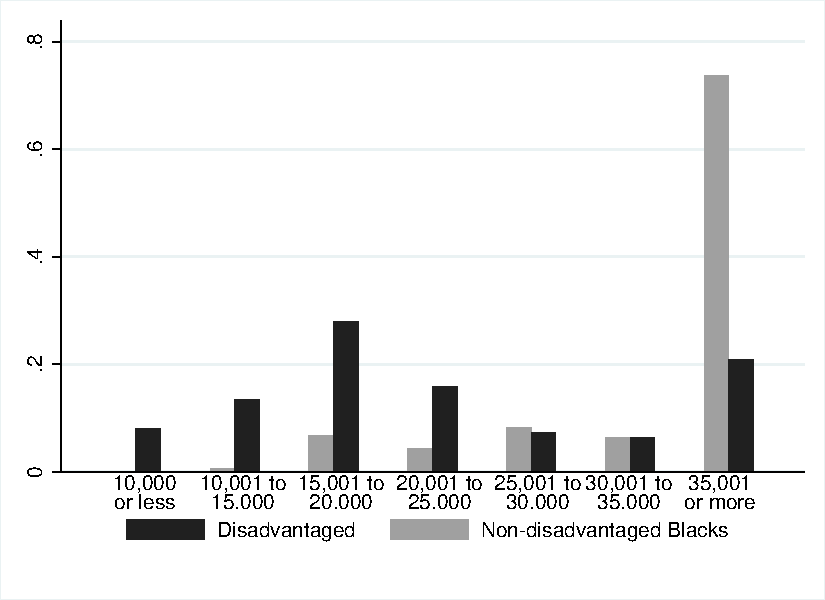
\includegraphics{abc_moink_b}}}
         \subfloat[Perry Birth Cohort]{
                \scalebox{0.7}{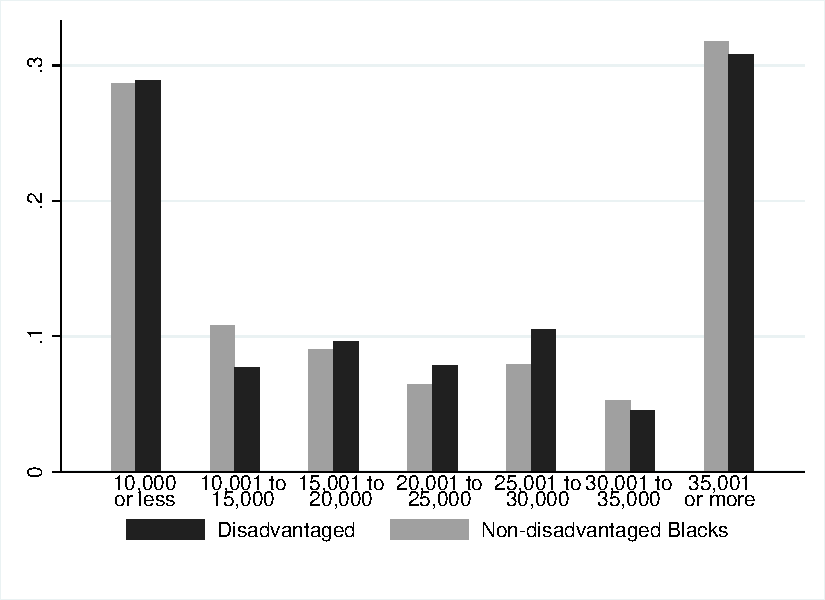
\includegraphics{perry_moink_b}}} \\
\end{center}
{\scriptsize {\bfseries Notes: } \raggedright 
Income is in 2010 dollars. The figures plot the frequency of family income, by disadvantage status and income block, for the ABC (1972 to 1977) and Perry (1957 to 1964) birth cohorts.  For the left plot we use PSID data. The PSID weights are used to make each sample representative  of its correlative in the population. Disadvantaged blacks meet the  ABC eligibility criteria as described in \citet{Ramey_Smith_1977_AJMD}. For the right plot, we use NLSY79 data. The NLSY weights are used to make each sample representative  of its correlative in the 1979 population. Disadvantaged blacks meet the Perry eligibility criteria as described in \citet{heckman2010analyzing}.
}
\end{figure}

\begin{figure} \begin{center}\centering
        \caption{Comparison of Disadvantaged Blacks and the Rest of the Population: Family Income}
        \label{graph:abc_moink_all}\vspace{0.2cm}
         \subfloat[ABC Birth Cohort]{
                \scalebox{0.7}{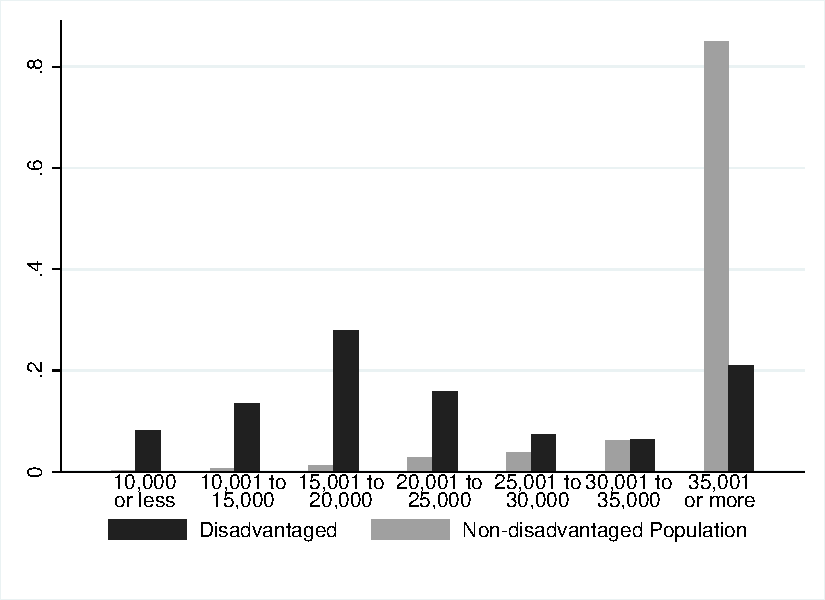
\includegraphics{abc_moink_all}}}
         \subfloat[Perry Birth Cohort]{
                \scalebox{0.7}{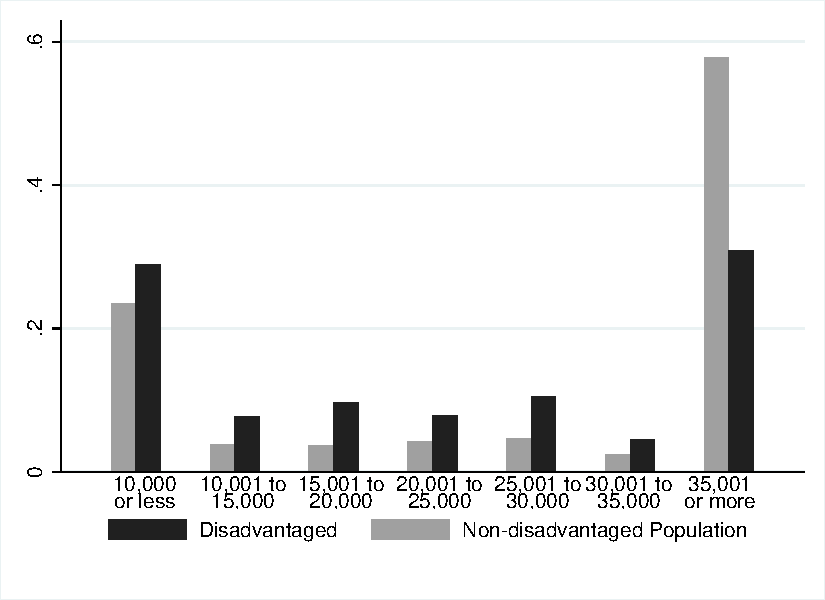
\includegraphics{perry_moink_all}}} \\
\end{center}
{\scriptsize {\bfseries Notes: } \raggedright 
Income is in 2010 dollars. The figures plot the frequency of family income, by disadvantage status and income block, for the ABC (1972 to 1977) and Perry (1957 to 1964) birth cohorts. For the left plot we use PSID data. 10\% of the cases had the years of education of the mother imputed in that survey. The PSID weights are used to make each sample representative  of its correlative in the population. Disadvantaged blacks meet the  ABC eligibility criteria as described in \citet{Ramey_Smith_1977_AJMD}. For the right plot, we use NLSY79 data. The NLSY weights are used to make each sample representative  of its correlative in the 1979 population. Disadvantaged blacks meet the Perry eligibility criteria as described in \citet{heckman2010analyzing}.
}
\end{figure}
\restoregeometry

